\documentclass[sigconf,review,anonymous]{acmart}
\providecommand{\tightlist}{\setlength{\itemsep}{0pt}\setlength{\parskip}{0pt}}
\setcopyright{none}
\usepackage{pgfplots}
\pgfplotsset{compat=1.18}
\usetikzlibrary{positioning,arrows.meta,calc}
\acmConference[MMSys '27]{ACM Multimedia Systems Conference}{2027}{}
\emergencystretch=3em
\sloppy
\begin{document}
\title{Structural Construction of Retrieval Graphs for Long-Video Question Answering}
\author{Anonymous Author(s)}
\affiliation{\institution{Anonymous Institution}\country{}}
\begin{abstract}
Graph-based pipelines for long-video question answering increasingly build their retrieval
graph with a large multimodal model, paying a generative cost per chunk that grows with
video duration. We build the graph structurally instead --- from compressed-domain signals and
CLIP embeddings, on CPU, with no generative model in the construction path --- and verify the
construction rather than benchmark it. A block-diagonal construction that enumerates only
within-scene node pairs is bit-identical to dense-then-prune construction (same nodes,
edges, weights at zero tolerance, and PageRank) while visiting 0.2\% of the pairs, making
construction \textasciitilde234\ensuremath{\times} faster and \textasciitilde6.8\ensuremath{\times} smaller in peak memory at 4,892 nodes. On the official
NExT-GQA test set the cheap graph shows no detected change in grounded accuracy against a dense
graph (+0.4 points, 95\% CI {[}\ensuremath{-}0.4, +1.2{]}, 5,553 questions). Query latency
separates with graph size --- exponent 2.06 (95\% CI {[}2.02, 2.13{]}) dense versus 0.83
({[}0.80, 0.88{]}) sparse --- and at the largest sizes tested only the sparse arm completes
within an hour. We also report where this does not help: a captioning stage dominates query time,
so a three-orders-of-magnitude retrieval speedup yields no end-to-end gain, and grounded
accuracy sits just below the weakly-supervised band (Acc@GQA 0.138 on the official test set,
\textasciitilde3.4B answerer on CPU). Two falsified hypotheses --- codec-derived scene boundaries and codec-based
frame admission, each tested against a stated kill criterion --- show that the block
structure, not the codec signal, carries the result.
\end{abstract}
\ccsdesc[500]{Information systems~Video search}
\ccsdesc[300]{Computing methodologies~Video summarization}
\keywords{long-video question answering, retrieval graphs, compressed-domain video, efficiency}
\maketitle
\section{Introduction}

Answering questions about long video requires structure. An hour of footage yields tens of
thousands of candidate frames, and flat retrieval over that pool becomes intractable before
it becomes inaccurate. The standard response is to build an intermediate graph over frames,
shots, or scenes and retrieve against it.

Increasingly, that graph is written by a large multimodal model: EgoSG prompts a proprietary
model per fixed-duration chunk, and Vgent extracts entities per clip with an LVLM. Both yield
richer representations than ours, but make construction model-metered and duration-scaled,
and the symbolic line rests on a proprietary model its authors report open models cannot
replace --- a poor foundation for footage that cannot leave the premises.

Two obvious claims are not ours. That construction cost is query-independent and amortises
across questions is Vgent's argument, measured before us; that compressed-domain signals
can stand in for full decode is older still (§2). Our contribution is narrower. We build the
graph with no generative model in the construction path --- a CLIP image encoder over
admitted frames is the only network --- and we verify the construction rather than benchmark
it.

\textbf{Construction.} The scene-sparse graph keeps only within-scene edges, yet the conventional
construction materialises the dense graph and prunes it: at N=4,892 admitted frames over 528
scenes it visits 11.96 million pairs to keep 23,571. Building the diagonal blocks directly
visits only the kept pairs and yields the same graph --- identical edges at tolerance 0.0,
bit-identical PageRank, identical retrieval on 406 questions --- in 0.212 s instead of 49.71 s
(\textasciitilde234\ensuremath{\times}) and 0.93 GB instead of 6.33 GB (\textasciitilde6.8\ensuremath{\times}). On the official NExT-GQA test set
it shows no detected change in grounded accuracy against the flat graph: +0.36 points,
95\% CI {[}\ensuremath{-}0.43, +1.17{]}, over 5,553 questions (§6.1).

\textbf{Scaling.} The same block structure changes how query cost grows. Over 19 clips under real
text queries, dense retrieval latency scales with graph size at exponent 2.063 (95\% CI
{[}2.020, 2.125{]}) and scene-sparse at 0.834 ({[}0.801, 0.884{]}). On the two largest clips
(6,559 and 13,506 admitted frames) the dense arm could not complete its measurement within an
hour, and at the larger its graph would, by extrapolation, exceed this machine's memory, while sparse
retrieval answered in 0.017 s and 0.029 s.

\textbf{What does not improve.} First, the retrieval speedup does not reach the user: at
N=4,892, retrieval falls from 8.535 s to 0.030 s, but captioning and verification, O(top\_k)
rather than O(N), take 44--67 s, and end to end the sparse arm is slower at the median
(0.802\ensuremath{\times}); we measure this rather than project a crossover (§5.3). Second, accuracy sits just
below the weakly-supervised band: on the official NExT-GQA test set, Acc@GQA is 0.138 with a
\textasciitilde3.4B answerer on CPU, and uniform sampling answers more questions correctly while rarely
grounding them (§6.1). We claim a correctness floor, not an advance.

\textbf{What does not matter.} We set kill criteria for two hypotheses we expected to confirm,
and both triggered. Codec-derived scene boundaries do not beat content-blind ones at matched
segment count (pre-registered; +0.088 M-Avg, 95\% CI {[}\ensuremath{-}0.009, +0.204{]} on long videos), and
codec-based frame admission is indistinguishable from uniform sampling at matched budget
(criterion set before any run). Neither where the
video is cut nor which frames are kept does the work; the block structure does. A pipeline
can therefore adopt the construction without our codec signal, segmentation, or admission
policy.

\textbf{Contributions.}

\begin{enumerate}
\def\labelenumi{\arabic{enumi}.}
\tightlist
\item
  A block-diagonal graph construction shown bit-identical to dense-then-prune, at \textasciitilde234\ensuremath{\times}
  lower build time and \textasciitilde6.8\ensuremath{\times} lower peak memory, with no detected change in grounded accuracy
  on the official NExT-GQA test set (§4, §6.1).
\item
  Query-latency scaling exponents with bootstrap confidence intervals over 19 clips, and
  measurements at sizes where the dense arm no longer completes (§5.1--§5.2).
\item
  A construction path with no generative model: frame selection performs zero neural
  forward passes, verified by instrumentation; full ingest costs 11.976 s per
  video, of which 2.845 s is selection (§3).
\item
  An Amdahl accounting of the query path, including a caption-cache locality cost that our
  sparse retrieval pays (§5.3--§5.4).
\item
  Two negative results under stated kill criteria, delimiting which components are
  load-bearing (§7).
\end{enumerate}

\section{Related Work}

\textbf{The token bottleneck.} At 1 FPS, published per-question frame budgets run from 32
(InternVL3~\cite{zhu2025internvl3}) and 180 (VideoLLaMA3~\cite{zhang2025videollama3}) to 512 (Qwen2.5-VL~\cite{bai2025qwen25vl}) and 3,900 frames (Gemini Flash
2.0~\cite{google2025gemini2flash}), against tens of thousands in an hour of footage. We build an intermediate
representation that later queries reuse, and retrieve per query against it.

\subsection{Graph-structured intermediate representations}

\textbf{EgoSG}~\cite{taluzzi2026egosg} partitions video into fixed 60 s chunks at 1 FPS and prompts
Gemini Flash 2.0 to emit a symbolic scene graph per chunk --- objects, spatial relations,
timestamped action hyperedges --- each chunk's graph produced by prompting the model to update
the previous one. On HD-EPIC~\cite{perrett2025hdepic} VQA it improves over raw-video input by 3.22 points for Gemini
itself and 5.60 for InternVL3-14B.

EgoSG's graph is a symbolic reasoning substrate and ours an embedding retrieval structure;
relational queries spanning a whole video genuinely favour the former, so we compare on
construction cost, not representational power.

Three properties of that construction matter. First, it is \textbf{model-metered and sequential}:
roughly 5.7 s per one-minute clip against a proprietary API, scaling linearly with duration,
and because chunk \(i\)'s graph depends on chunk \(i-1\)'s it cannot be parallelised across a
long video. The authors further report that open-source substitutes struggle to produce
accurate graphs reliably, and name that dependency as a limitation. Our scenes are
independent, so the block structure is parallel by definition, and no model participates in
construction.

Second, \textbf{no correctness guarantee is available for the artifact}: auditing five clips,
the authors find about 5\% of nodes and relations in error, 15.5\% false action hyperedges and
13.7\% of objects missing, and note that generation quality is not their focus --- expected of
a generative construction, not a criticism. A structural construction can be verified exactly
(§4.1), though only as \emph{fidelity} to our own dense-then-prune reference, not semantic
correctness: it cannot hallucinate an object, but neither can it recognise one.

\textbf{Vgent}~\cite{shen2025vgent} is the closer foil. It extracts entities per 64-frame clip with an LVLM and
links clips sharing them, on the same amortisation argument we make, and reports the split:
20.13 s of query-independent construction and 3.93 s of query-dependent work per minute of
video, against 20.81 s for Video-RAG~\cite{luo2024videorag}, a claimed 1.73\ensuremath{\times} speedup on VideoMME~\cite{fu2025videomme}. We are
not the first to measure construction cost separately.

Where we differ is what construction costs: our selection runs on CPU with zero neural forward
passes, and our only construction-time network is an image encoder (§3). \textbf{We draw no cost
ratio against these systems}: Vgent's 20.13 s is per \emph{minute of video} and includes LVLM
extraction, our 11.976 s is per video, and the honest claim concerns the \emph{class} of model.

Three further systems --- \textbf{EGAgent}~\cite{rege2026egagent}, \textbf{MemDreamer}~\cite{chen2026memdreamer}
and \textbf{GraphVideoAgent}~\cite{chu2025graphvideoagent} --- build their graphs with an LLM extractor,
a Gemini-3.1-Pro extractor, or by parsing a captioning model's output, so each places a
generative pass inside construction or one step upstream of it. None reports a
construction cost in a form comparable to ours, so no ratio comparison is available; the claim is about model
class only.

\subsection{Grounded video QA, and the accuracy frontier}

\textbf{NExT-GQA}~\cite{xiao2024nextgqa} requires that a system answer correctly \emph{and} point at its
evidence, reporting Acc@GQA alongside mIoP, IoP@0.5 and mIoU. Its finding that strong
answerers often ground poorly --- right for the wrong reasons --- is why we report grounded
accuracy rather than answer accuracy alone (§6). The weakly-supervised band there is occupied
by Temp{[}CLIP{]} with NG+ (16.0 Acc@GQA)~\cite{xiao2024nextgqa}, SeViLA~\cite{yu2023sevila} as reproduced by the benchmark authors (16.6),
LangRepo~\cite{kahatapitiya2024langrepo} (17.1) and FrozenBiLM~\cite{yang2022frozenbilm} with NG+ (17.5). Our §6.1 rows use the same full
5,553-question test set.

A more recent line attaches an explicit temporal grounder, often with cooperating agents:
\textbf{MUPA}~\cite{dang2025mupa} reports 28.7 Acc@GQA at 2B and 30.3 at 7B, \textbf{VideoMind}~\cite{liu2025videomind} 25.2 at 2B. These define
the current frontier. We do not compete with them on accuracy --- our contribution is
construction cost and our answer quality sits a band below (§6) --- and cite them to situate
that gap rather than to select a weaker comparison set.

\subsection{Compressed-domain video analysis}

Using bitstream signals --- motion vectors, residual energy, packet size --- to avoid full decode
is long-standing, running from motion-vector surrogates for optical flow~\cite{zhang2016mvcnn}
through CoViAR~\cite{wu2018coviar} and DMC-Net~\cite{shou2019dmcnet}. It has recently reached video language models:
\textbf{CoPE-VideoLM}~\cite{sarkar2026cope} converts each P-frame into eight compact \ensuremath{\Delta}-tokens from
its motion vectors and residuals, reporting up to 86\% lower time-to-first-token and up to 93\%
fewer visual tokens across 14 benchmarks.

Our use of the codec differs in kind, and that distinction is what makes our negative result
compatible with their positive one. CoPE-VideoLM uses codec primitives as a \emph{representation},
encoded and consumed by the model, at the cost of a trained \ensuremath{\Delta}-encoder and end-to-end
fine-tuning. We use codec statistics as a \emph{selection and weighting heuristic} over frames we
then treat conventionally, training nothing. That codec-derived salience does not beat
uniform sampling for \emph{admission} (§7.2) says nothing about whether the same fields carry
signal when \emph{encoded}; we take no position on theirs.

Our claim is correspondingly modest, and §7 constrains it: compressed-domain signals here
are a \emph{cheap} source of structure, not an \emph{informative} one.

\subsection{Positioning}

Against EgoSG and its family we replace a frontier-model-generated symbolic graph with a
structurally-constructed one: built with no generative model, verifiable, parallel, locally
runnable --- and semantically poorer. Against grounded-QA baselines we land just below the weakly-supervised band
while training nothing and running on CPU; against the agentic frontier we are a band behind
on accuracy. The claim is narrow: for
retrieval over long video, the intermediate graph does not have to be expensive, and does not
have to be generated.

\section{Method}

\begin{figure*}[t]
\centering
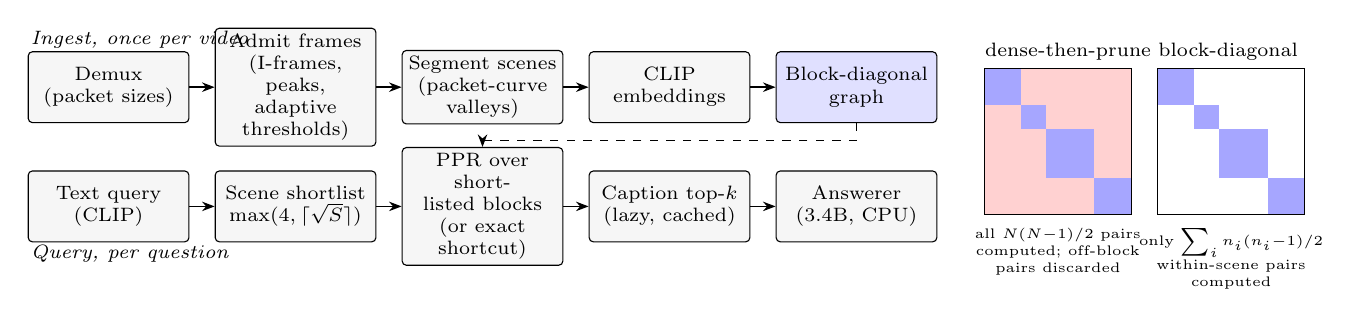
\begin{tikzpicture}[font=\scriptsize,
  box/.style={draw, rounded corners=1.5pt, align=center, minimum height=9mm, text width=19mm, inner sep=2pt, fill=gray!7},
  hot/.style={box, fill=blue!12},
  arr/.style={-{Stealth[length=1.6mm]}, semithick}]
\node[box] (demux) {Demux\\(packet sizes)};
\node[box, right=3.2mm of demux] (admit) {Admit frames\\(I-frames, peaks,\\adaptive thresholds)};
\node[box, right=3.2mm of admit] (scenes) {Segment scenes\\(packet-curve\\valleys)};
\node[box, right=3.2mm of scenes] (clip) {CLIP\\embeddings};
\node[hot, right=3.2mm of clip] (graph) {Block-diagonal\\graph};
\foreach \a/\b in {demux/admit, admit/scenes, scenes/clip, clip/graph} \draw[arr] (\a) -- (\b);
\node[box, below=6mm of demux] (q) {Text query\\(CLIP)};
\node[box, right=3.2mm of q] (short) {Scene shortlist\\$\max(4,\lceil\sqrt{S}\rceil)$};
\node[box, right=3.2mm of short] (ppr) {PPR over short-\\listed blocks\\(or exact shortcut)};
\node[box, right=3.2mm of ppr] (cap) {Caption top-$k$\\(lazy, cached)};
\node[box, right=3.2mm of cap] (ans) {Answerer\\(3.4B, CPU)};
\foreach \a/\b in {q/short, short/ppr, ppr/cap, cap/ans} \draw[arr] (\a) -- (\b);
\draw[arr, dashed] (graph.south) -- ++(0,-2.2mm) -| (ppr.north);
\node[anchor=south west, font=\scriptsize\itshape, inner sep=1pt] at (demux.north west) {Ingest, once per video};
\node[anchor=north west, font=\scriptsize\itshape, inner sep=1pt] at (q.south west) {Query, per question};
% adjacency matrices
\def\s{0.155}
\begin{scope}[shift={($(graph.east)+(6mm,-1.62)$)}]
  \node[anchor=south west, font=\scriptsize, inner sep=0pt] at (0,1.95) {dense-then-prune};
  \fill[red!18] (0,0) rectangle (12*\s,12*\s);
  \foreach \o/\n in {0/3,3/2,5/4,9/3} \fill[blue!35] (\o*\s,12*\s-\o*\s) rectangle ({(\o+\n)*\s},{12*\s-(\o+\n)*\s});
  \draw (0,0) rectangle (12*\s,12*\s);
  \node[font=\tiny, align=center, anchor=north] at (6*\s,-0.05) {all $N(N{-}1)/2$ pairs\\computed; off-block\\pairs discarded};
\end{scope}
\begin{scope}[shift={($(graph.east)+(6mm+22mm,-1.62)$)}]
  \node[anchor=south west, font=\scriptsize, inner sep=0pt] at (0,1.95) {block-diagonal};
  \foreach \o/\n in {0/3,3/2,5/4,9/3} \fill[blue!35] (\o*\s,12*\s-\o*\s) rectangle ({(\o+\n)*\s},{12*\s-(\o+\n)*\s});
  \draw (0,0) rectangle (12*\s,12*\s);
  \node[font=\tiny, align=center, anchor=north] at (6*\s,-0.05) {only $\sum_i n_i(n_i{-}1)/2$\\within-scene pairs\\computed};
\end{scope}
\end{tikzpicture}
\Description{Two rows of pipeline boxes. Ingest: demux packet sizes, admit frames, segment scenes, CLIP embeddings, block-diagonal graph. Query: text query, scene shortlist, personalised PageRank over shortlisted blocks or an exact shortcut, lazy captioning of the top k frames, answerer. At right, two 12-by-12 adjacency grids: dense-then-prune computes every cell and discards the off-diagonal ones; block-diagonal computes only the diagonal blocks.}
\caption{IRIS in one view. Right: dense-then-prune computes every pair and discards those across scenes (red); block-diagonal construction computes only the within-scene blocks (blue), yielding the identical graph (\S4.1).}
\label{fig:overview}
\end{figure*}

IRIS ingests a video once into a compact index, then answers arbitrary text queries against
it (Figure~\ref{fig:overview}). Throughout, \textbf{N} denotes the number of \emph{surviving} frames after admission, not the frame
count in the container --- the distinction matters for every scaling figure we report.

\subsection{Ingest and frame admission}

Ingest demuxes the video and admits frames from the packet-size curve alone: I-frames and
packet-curve peaks are always kept, and any other frame is kept when its packet size clears
adaptive thresholds set per keyframe interval (\texttt{salient\_thresh} 0.35, \texttt{candidate\_thresh} 0.08
before adaptation). Packet size stands in for the residual signal because it is what the decoder API
exposes: libavcodec exposes motion vectors as side data (\texttt{EXPORT\_MVS}) but no
coefficient-level residual, per-block quantisation parameter or reconstruction-error signal.
Admitted frames --- the survivors --- are the input to everything downstream; on the annotated
corpus they are 10.41--11.14\% of frames. Each survivor then receives a scalar \textbf{action
score} combining the packet-size residual, motion energy and luma entropy at weights 0.5 / 0.3 /
0.2; the score enters edge weights (§3.6) but does not decide admission.

\textbf{No neural network runs during frame selection.} We verify this by instrumentation rather
than inspection: monkeypatching \texttt{torch.nn.Module.\_\_call\_\_} for the duration of every
\texttt{parse\_video()} call and counting invocations across 32 videos yields exactly zero.

CLIP~\cite{radford2021clip} embeddings (ViT-B/32) are computed for admitted frames \emph{after} that stage, and are what
the zero-forward-pass claim excludes. Captioning is deferred entirely; \texttt{caption} remains
\texttt{None} at ingest. Over the same frozen 32-video sample, selection (\texttt{parse\_video}) takes
2.845 s per video (range 0.314--14.870 s), CLIP enrichment 9.131 s (0.501--56.885 s), and full
ingest \textbf{11.976 s} (0.814--71.754 s).

CLIP enrichment, at 26.56 ms per admitted frame, costs roughly three times the selection stage.
\textbf{The honest headline for construction is therefore \textasciitilde12 s per video, not \textasciitilde2.9 s.} Our ingest
as a whole is \emph{not} forward-pass-free; the smaller figure describes the forward-pass-free
portion only, and any comparison against a system whose reported construction cost includes
its neural extraction stage is not like-for-like on it. Selection-stage peak RSS is 530 MB
mean, measured in a run where torch was never loaded.

\subsection{Scene segmentation}

\begin{figure}[t]
\centering
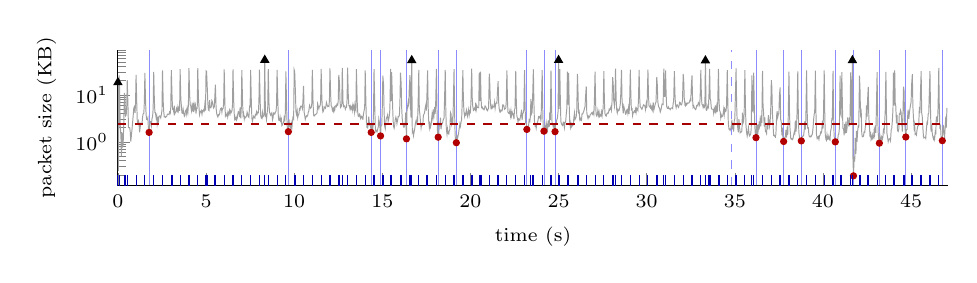
\begin{tikzpicture}
\begin{semilogyaxis}[width=\columnwidth, height=3.3cm, font=\scriptsize, xmin=0, xmax=47.1, ymin=0.12, ymax=90,
  xlabel={time (s)}, ylabel={packet size (KB)}, ytick={0.1,1,10,100}, axis lines*=left, clip=true]
\draw[blue!45, line width=0.3pt] (axis cs:1.77,0.12) -- (axis cs:1.77,90);
\draw[blue!45, line width=0.3pt] (axis cs:9.67,0.12) -- (axis cs:9.67,90);
\draw[blue!45, line width=0.3pt] (axis cs:14.37,0.12) -- (axis cs:14.37,90);
\draw[blue!45, line width=0.3pt] (axis cs:14.90,0.12) -- (axis cs:14.90,90);
\draw[blue!45, line width=0.3pt] (axis cs:16.37,0.12) -- (axis cs:16.37,90);
\draw[blue!45, line width=0.3pt] (axis cs:18.17,0.12) -- (axis cs:18.17,90);
\draw[blue!45, line width=0.3pt] (axis cs:19.20,0.12) -- (axis cs:19.20,90);
\draw[blue!45, line width=0.3pt] (axis cs:23.20,0.12) -- (axis cs:23.20,90);
\draw[blue!45, line width=0.3pt] (axis cs:24.17,0.12) -- (axis cs:24.17,90);
\draw[blue!45, line width=0.3pt] (axis cs:24.80,0.12) -- (axis cs:24.80,90);
\draw[blue!45, line width=0.3pt] (axis cs:36.20,0.12) -- (axis cs:36.20,90);
\draw[blue!45, line width=0.3pt] (axis cs:37.77,0.12) -- (axis cs:37.77,90);
\draw[blue!45, line width=0.3pt] (axis cs:38.77,0.12) -- (axis cs:38.77,90);
\draw[blue!45, line width=0.3pt] (axis cs:40.70,0.12) -- (axis cs:40.70,90);
\draw[blue!45, line width=0.3pt] (axis cs:41.73,0.12) -- (axis cs:41.73,90);
\draw[blue!45, line width=0.3pt] (axis cs:43.20,0.12) -- (axis cs:43.20,90);
\draw[blue!45, line width=0.3pt] (axis cs:44.70,0.12) -- (axis cs:44.70,90);
\draw[blue!45, line width=0.3pt] (axis cs:46.77,0.12) -- (axis cs:46.77,90);
\draw[blue!45, line width=0.5pt, dashed] (axis cs:34.80,0.12) -- (axis cs:34.80,90);
\addplot[gray!75, line width=0.35pt] coordinates {(0.00,18.32) (0.03,0.24) (0.07,25.85) (0.10,11.97) (0.13,2.31) (0.17,1.32) (0.20,0.49) (0.23,1.62) (0.27,0.76) (0.30,0.98) (0.33,2.22) (0.37,10.96) (0.40,8.51) (0.43,3.56) (0.47,3.75) (0.50,5.62) (0.53,20.40) (0.57,6.12) (0.60,2.04) (0.63,1.99) (0.67,2.01) (0.70,1.64) (0.73,1.02) (0.77,1.42) (0.80,1.85) (0.83,2.48) (0.87,3.75) (0.90,5.23) (0.93,5.53) (0.97,4.10) (1.00,6.50) (1.03,26.47) (1.07,6.52) (1.10,2.65) (1.13,2.52) (1.17,2.80) (1.20,2.41) (1.23,1.59) (1.27,2.11) (1.30,2.46) (1.33,2.38) (1.37,2.50) (1.40,3.39) (1.43,3.94) (1.47,4.03) (1.50,7.03) (1.53,29.23) (1.57,6.93) (1.60,3.76) (1.63,3.00) (1.67,2.95) (1.70,3.23) (1.73,1.94) (1.77,1.59) (1.80,2.35) (1.83,2.73) (1.87,2.69) (1.90,2.21) (1.93,3.05) (1.97,3.56) (2.00,5.08) (2.03,30.81) (2.07,7.18) (2.10,4.17) (2.13,4.17) (2.17,3.24) (2.20,3.57) (2.23,2.41) (2.27,3.07) (2.30,2.75) (2.33,3.51) (2.37,3.56) (2.40,3.53) (2.43,3.26) (2.47,3.87) (2.50,4.74) (2.53,33.20) (2.57,7.14) (2.60,4.36) (2.63,3.40) (2.67,3.47) (2.70,3.32) (2.73,3.39) (2.77,3.49) (2.80,3.81) (2.83,3.90) (2.87,3.88) (2.90,3.81) (2.93,4.30) (2.97,4.05) (3.00,5.45) (3.03,33.53) (3.07,9.72) (3.10,5.00) (3.13,5.11) (3.17,4.30) (3.20,5.87) (3.23,3.97) (3.27,4.29) (3.30,4.35) (3.33,5.13) (3.37,4.57) (3.40,5.49) (3.43,4.57) (3.47,5.38) (3.50,4.57) (3.53,35.19) (3.57,8.00) (3.60,5.89) (3.63,4.13) (3.67,4.05) (3.70,4.95) (3.73,4.17) (3.77,3.49) (3.80,3.64) (3.83,4.49) (3.87,4.79) (3.90,3.98) (3.93,5.16) (3.97,4.23) (4.00,6.13) (4.03,36.74) (4.07,9.89) (4.10,6.17) (4.13,5.85) (4.17,4.62) (4.20,5.75) (4.23,4.48) (4.27,6.72) (4.30,4.29) (4.33,6.25) (4.37,5.21) (4.40,5.96) (4.43,4.00) (4.47,5.25) (4.50,5.19) (4.53,36.87) (4.57,8.31) (4.60,5.41) (4.63,3.79) (4.67,4.42) (4.70,4.35) (4.73,4.62) (4.77,3.85) (4.80,4.54) (4.83,4.42) (4.87,4.86) (4.90,4.59) (4.93,6.17) (4.97,4.62) (5.00,32.37) (5.03,31.64) (5.07,14.08) (5.10,6.89) (5.13,4.87) (5.17,4.63) (5.20,7.66) (5.23,5.34) (5.27,5.28) (5.30,5.66) (5.33,7.53) (5.37,7.03) (5.40,5.73) (5.43,5.25) (5.47,5.63) (5.50,9.30) (5.53,16.51) (5.57,5.27) (5.60,4.11) (5.63,3.65) (5.67,3.40) (5.70,3.78) (5.73,3.68) (5.77,3.92) (5.80,4.77) (5.83,5.10) (5.87,5.23) (5.90,4.30) (5.93,5.10) (5.97,5.12) (6.00,6.72) (6.03,34.57) (6.07,6.31) (6.10,3.56) (6.13,3.81) (6.17,3.60) (6.20,4.09) (6.23,3.40) (6.27,4.13) (6.30,3.88) (6.33,4.68) (6.37,4.01) (6.40,4.53) (6.43,4.23) (6.47,4.55) (6.50,6.06) (6.53,34.90) (6.57,7.17) (6.60,3.92) (6.63,2.91) (6.67,2.99) (6.70,3.38) (6.73,2.92) (6.77,3.18) (6.80,3.87) (6.83,4.38) (6.87,4.23) (6.90,3.38) (6.93,5.37) (6.97,3.18) (7.00,5.20) (7.03,33.59) (7.07,7.47) (7.10,3.73) (7.13,4.04) (7.17,3.03) (7.20,3.39) (7.23,3.26) (7.27,3.40) (7.30,3.58) (7.33,4.28) (7.37,3.81) (7.40,3.40) (7.43,3.31) (7.47,5.65) (7.50,5.52) (7.53,33.75) (7.57,6.94) (7.60,3.19) (7.63,2.74) (7.67,3.19) (7.70,3.50) (7.73,3.29) (7.77,3.20) (7.80,3.79) (7.83,3.70) (7.87,4.39) (7.90,3.93) (7.93,4.20) (7.97,4.15) (8.00,7.42) (8.03,34.41) (8.07,7.31) (8.10,3.68) (8.13,3.23) (8.17,3.12) (8.20,4.16) (8.23,3.42) (8.27,3.60) (8.30,3.80) (8.33,54.88) (8.37,3.60) (8.40,3.75) (8.43,3.00) (8.47,4.20) (8.50,5.52) (8.53,35.09) (8.57,6.78) (8.60,4.33) (8.63,3.98) (8.67,3.69) (8.70,3.98) (8.73,4.15) (8.77,2.95) (8.80,3.26) (8.83,4.12) (8.87,4.11) (8.90,3.91) (8.93,4.22) (8.97,4.50) (9.00,5.94) (9.03,33.91) (9.07,7.94) (9.10,3.50) (9.13,2.87) (9.17,2.84) (9.20,3.38) (9.23,2.79) (9.27,3.09) (9.30,2.22) (9.33,2.29) (9.37,2.50) (9.40,2.60) (9.43,3.30) (9.47,2.91) (9.50,4.24) (9.53,31.64) (9.57,5.82) (9.60,2.28) (9.63,1.72) (9.67,1.65) (9.70,3.08) (9.73,2.38) (9.77,2.08) (9.80,1.98) (9.83,2.51) (9.87,1.99) (9.90,2.58) (9.93,3.31) (9.97,3.08) (10.00,34.06) (10.03,31.11) (10.07,11.57) (10.10,4.47) (10.13,3.85) (10.17,4.61) (10.20,3.27) (10.23,3.67) (10.27,3.94) (10.30,5.04) (10.33,4.86) (10.37,5.77) (10.40,5.77) (10.43,5.64) (10.47,5.06) (10.50,7.95) (10.53,15.57) (10.57,4.16) (10.60,3.62) (10.63,3.01) (10.67,3.35) (10.70,3.56) (10.73,3.46) (10.77,3.68) (10.80,4.29) (10.83,4.50) (10.87,5.92) (10.90,5.45) (10.93,5.17) (10.97,5.45) (11.00,6.59) (11.03,33.92) (11.07,7.12) (11.10,3.76) (11.13,3.54) (11.17,3.66) (11.20,3.86) (11.23,3.85) (11.27,3.98) (11.30,4.14) (11.33,6.47) (11.37,5.65) (11.40,5.07) (11.43,5.68) (11.47,5.83) (11.50,6.98) (11.53,35.36) (11.57,8.50) (11.60,5.22) (11.63,4.31) (11.67,4.62) (11.70,5.55) (11.73,5.38) (11.77,5.17) (11.80,5.75) (11.83,6.88) (11.87,6.04) (11.90,5.67) (11.93,5.82) (11.97,5.66) (12.00,7.42) (12.03,36.28) (12.07,9.70) (12.10,5.81) (12.13,5.64) (12.17,4.68) (12.20,5.07) (12.23,4.48) (12.27,5.31) (12.30,4.75) (12.33,5.64) (12.37,5.93) (12.40,5.66) (12.43,6.32) (12.47,6.05) (12.50,7.58) (12.53,26.59) (12.57,18.26) (12.60,7.34) (12.63,5.37) (12.67,5.61) (12.70,6.42) (12.73,37.50) (12.77,7.20) (12.80,5.59) (12.83,5.71) (12.87,5.82) (12.90,4.97) (12.93,5.37) (12.97,5.45) (13.00,7.89) (13.03,37.62) (13.07,9.84) (13.10,5.88) (13.13,5.91) (13.17,4.95) (13.20,5.64) (13.23,5.08) (13.27,5.56) (13.30,4.71) (13.33,6.02) (13.37,5.10) (13.40,6.02) (13.43,4.30) (13.47,5.64) (13.50,5.03) (13.53,34.97) (13.57,8.03) (13.60,4.48) (13.63,3.54) (13.67,3.44) (13.70,3.90) (13.73,3.80) (13.77,3.17) (13.80,3.46) (13.83,3.52) (13.87,3.07) (13.90,3.03) (13.93,3.91) (13.97,4.66) (14.00,5.37) (14.03,33.11) (14.07,6.55) (14.10,2.66) (14.13,2.03) (14.17,1.98) (14.20,2.39) (14.23,3.44) (14.27,2.44) (14.30,2.22) (14.33,2.21) (14.37,1.59) (14.40,2.44) (14.43,1.68) (14.47,2.02) (14.50,4.07) (14.53,35.04) (14.57,6.13) (14.60,2.14) (14.63,1.64) (14.67,1.73) (14.70,1.63) (14.73,1.78) (14.77,2.10) (14.80,3.06) (14.83,2.65) (14.87,1.96) (14.90,1.34) (14.93,2.24) (14.97,2.29) (15.00,5.67) (15.03,25.59) (15.07,16.61) (15.10,4.73) (15.13,2.17) (15.17,1.90) (15.20,2.69) (15.23,3.19) (15.27,3.40) (15.30,3.73) (15.33,2.73) (15.37,3.12) (15.40,3.64) (15.43,5.00) (15.47,35.62) (15.50,7.39) (15.53,30.20) (15.57,8.90) (15.60,3.85) (15.63,2.21) (15.67,1.95) (15.70,2.21) (15.73,2.88) (15.77,3.35) (15.80,3.04) (15.83,2.45) (15.87,2.92) (15.90,3.45) (15.93,3.41) (15.97,3.71) (16.00,7.16) (16.03,29.55) (16.07,17.29) (16.10,5.22) (16.13,3.11) (16.17,2.42) (16.20,2.11) (16.23,2.04) (16.27,2.22) (16.30,2.63) (16.33,4.23) (16.37,1.16) (16.40,4.51) (16.43,5.57) (16.47,7.12) (16.50,6.16) (16.53,13.69) (16.57,26.26) (16.60,6.13) (16.63,3.27) (16.67,53.96) (16.70,1.63) (16.73,1.76) (16.77,1.36) (16.80,1.59) (16.83,1.78) (16.87,2.38) (16.90,2.71) (16.93,2.49) (16.97,3.10) (17.00,2.79) (17.03,6.09) (17.07,34.04) (17.10,4.79) (17.13,3.92) (17.17,2.58) (17.20,1.99) (17.23,2.38) (17.27,2.27) (17.30,2.33) (17.33,3.65) (17.37,3.92) (17.40,4.22) (17.43,5.21) (17.47,6.12) (17.50,4.61) (17.53,9.49) (17.57,33.07) (17.60,5.76) (17.63,2.84) (17.67,2.00) (17.70,2.40) (17.73,2.05) (17.77,2.35) (17.80,3.12) (17.83,4.08) (17.87,3.13) (17.90,4.16) (17.93,3.60) (17.97,5.51) (18.00,3.94) (18.03,7.13) (18.07,35.36) (18.10,5.39) (18.13,1.66) (18.17,1.26) (18.20,1.40) (18.23,2.24) (18.27,2.20) (18.30,3.27) (18.33,1.86) (18.37,2.38) (18.40,2.41) (18.43,2.65) (18.47,3.09) (18.50,3.13) (18.53,7.65) (18.57,33.74) (18.60,5.27) (18.63,1.92) (18.67,1.45) (18.70,1.88) (18.73,1.54) (18.77,1.47) (18.80,1.73) (18.83,1.83) (18.87,4.19) (18.90,3.90) (18.93,2.45) (18.97,3.00) (19.00,2.38) (19.03,6.54) (19.07,35.28) (19.10,4.50) (19.13,1.39) (19.17,0.97) (19.20,0.96) (19.23,1.33) (19.27,1.20) (19.30,1.36) (19.33,1.55) (19.37,2.03) (19.40,2.41) (19.43,2.15) (19.47,2.67) (19.50,2.99) (19.53,6.52) (19.57,33.57) (19.60,8.12) (19.63,4.50) (19.67,3.48) (19.70,3.94) (19.73,3.79) (19.77,4.71) (19.80,3.98) (19.83,3.52) (19.87,4.39) (19.90,4.97) (19.93,3.69) (19.97,4.49) (20.00,4.30) (20.03,7.53) (20.07,36.19) (20.10,8.77) (20.13,5.77) (20.17,4.65) (20.20,4.77) (20.23,5.14) (20.27,4.82) (20.30,6.78) (20.33,4.81) (20.37,5.77) (20.40,5.39) (20.43,5.41) (20.47,5.31) (20.50,29.49) (20.53,7.44) (20.57,31.16) (20.60,8.57) (20.63,5.35) (20.67,5.50) (20.70,5.06) (20.73,5.13) (20.77,4.82) (20.80,5.13) (20.83,5.79) (20.87,5.54) (20.90,5.24) (20.93,4.73) (20.97,4.57) (21.00,5.00) (21.03,5.24) (21.07,28.23) (21.10,16.22) (21.13,6.85) (21.17,5.03) (21.20,5.04) (21.23,5.97) (21.27,5.37) (21.30,5.64) (21.33,5.58) (21.37,6.97) (21.40,5.20) (21.43,6.36) (21.47,6.71) (21.50,6.65) (21.53,11.03) (21.57,19.54) (21.60,6.96) (21.63,5.13) (21.67,4.29) (21.70,4.29) (21.73,4.74) (21.77,4.57) (21.80,4.58) (21.83,6.09) (21.87,6.08) (21.90,5.74) (21.93,4.96) (21.97,5.11) (22.00,5.09) (22.03,6.96) (22.07,32.88) (22.10,7.57) (22.13,4.24) (22.17,4.05) (22.20,4.00) (22.23,4.53) (22.27,3.56) (22.30,4.55) (22.33,3.56) (22.37,4.24) (22.40,3.83) (22.43,3.90) (22.47,3.05) (22.50,4.92) (22.53,5.16) (22.57,32.14) (22.60,7.88) (22.63,3.56) (22.67,3.19) (22.70,2.66) (22.73,3.09) (22.77,3.01) (22.80,2.90) (22.83,3.33) (22.87,4.03) (22.90,4.81) (22.93,2.89) (22.97,3.98) (23.00,4.19) (23.03,4.89) (23.07,33.62) (23.10,5.62) (23.13,2.51) (23.17,2.49) (23.20,1.84) (23.23,2.03) (23.27,2.07) (23.30,2.26) (23.33,2.92) (23.37,2.74) (23.40,3.43) (23.43,8.19) (23.47,4.00) (23.50,4.27) (23.53,9.41) (23.57,34.92) (23.60,7.09) (23.63,2.78) (23.67,2.18) (23.70,2.26) (23.73,1.95) (23.77,2.47) (23.80,2.55) (23.83,2.83) (23.87,3.46) (23.90,3.43) (23.93,3.27) (23.97,3.54) (24.00,2.69) (24.03,6.57) (24.07,33.63) (24.10,5.28) (24.13,1.79) (24.17,1.69) (24.20,1.75) (24.23,2.30) (24.27,1.76) (24.30,2.03) (24.33,2.51) (24.37,1.79) (24.40,2.12) (24.43,2.87) (24.47,2.08) (24.50,4.26) (24.53,2.90) (24.57,32.96) (24.60,5.69) (24.63,2.50) (24.67,2.34) (24.70,2.06) (24.73,2.26) (24.77,2.22) (24.80,1.65) (24.83,2.31) (24.87,2.53) (24.90,2.95) (24.93,3.16) (24.97,4.37) (25.00,54.39) (25.03,5.06) (25.07,35.27) (25.10,7.92) (25.13,2.69) (25.17,2.40) (25.20,2.28) (25.23,2.22) (25.27,2.63) (25.30,2.60) (25.33,2.02) (25.37,2.61) (25.40,2.64) (25.43,3.65) (25.47,5.21) (25.50,31.27) (25.53,6.16) (25.57,29.09) (25.60,6.70) (25.63,2.73) (25.67,2.06) (25.70,2.50) (25.73,2.08) (25.77,2.24) (25.80,2.21) (25.83,2.30) (25.87,3.31) (25.90,4.09) (25.93,2.98) (25.97,3.20) (26.00,3.42) (26.03,4.59) (26.07,27.86) (26.10,12.73) (26.13,4.25) (26.17,4.52) (26.20,2.99) (26.23,3.18) (26.27,2.82) (26.30,2.83) (26.33,3.95) (26.37,3.92) (26.40,4.27) (26.43,4.46) (26.47,5.19) (26.50,5.58) (26.53,9.07) (26.57,15.04) (26.60,4.15) (26.63,3.65) (26.67,3.15) (26.70,3.49) (26.73,3.30) (26.77,3.49) (26.80,3.81) (26.83,3.87) (26.87,4.09) (26.90,4.21) (26.93,3.90) (26.97,4.27) (27.00,3.86) (27.03,6.74) (27.07,31.21) (27.10,6.84) (27.13,3.81) (27.17,3.53) (27.20,3.79) (27.23,4.69) (27.27,3.67) (27.30,4.22) (27.33,3.46) (27.37,3.72) (27.40,3.57) (27.43,4.38) (27.47,3.63) (27.50,4.61) (27.53,5.10) (27.57,31.72) (27.60,7.25) (27.63,4.03) (27.67,3.60) (27.70,3.51) (27.73,3.88) (27.77,4.10) (27.80,4.01) (27.83,4.15) (27.87,4.95) (27.90,4.75) (27.93,4.99) (27.97,5.56) (28.00,4.80) (28.03,6.87) (28.07,23.83) (28.10,16.93) (28.13,7.49) (28.17,5.77) (28.20,8.36) (28.23,35.89) (28.27,7.46) (28.30,4.72) (28.33,4.11) (28.37,4.87) (28.40,4.58) (28.43,4.65) (28.47,5.31) (28.50,6.38) (28.53,10.65) (28.57,34.07) (28.60,7.95) (28.63,5.63) (28.67,4.06) (28.70,5.71) (28.73,5.10) (28.77,4.47) (28.80,3.90) (28.83,3.95) (28.87,4.79) (28.90,4.89) (28.93,4.08) (28.97,5.36) (29.00,3.90) (29.03,6.55) (29.07,34.11) (29.10,10.32) (29.13,4.84) (29.17,4.99) (29.20,3.63) (29.23,4.14) (29.27,4.32) (29.30,4.54) (29.33,4.29) (29.37,5.03) (29.40,4.26) (29.43,5.20) (29.47,4.90) (29.50,4.64) (29.53,7.43) (29.57,33.84) (29.60,8.76) (29.63,5.62) (29.67,5.34) (29.70,5.14) (29.73,4.92) (29.77,5.47) (29.80,5.81) (29.83,6.15) (29.87,5.97) (29.90,5.68) (29.93,4.87) (29.97,6.38) (30.00,5.25) (30.03,8.29) (30.07,34.40) (30.10,9.82) (30.13,5.81) (30.17,5.61) (30.20,5.34) (30.23,6.05) (30.27,5.01) (30.30,5.43) (30.33,4.84) (30.37,6.90) (30.40,4.69) (30.43,5.22) (30.47,6.07) (30.50,6.66) (30.53,7.08) (30.57,24.05) (30.60,16.64) (30.63,7.09) (30.67,5.72) (30.70,5.35) (30.73,5.16) (30.77,4.31) (30.80,4.67) (30.83,5.25) (30.87,6.38) (30.90,6.33) (30.93,6.24) (30.97,35.94) (31.00,9.26) (31.03,9.21) (31.07,32.98) (31.10,10.80) (31.13,5.75) (31.17,5.16) (31.20,5.10) (31.23,5.53) (31.27,5.08) (31.30,5.08) (31.33,4.83) (31.37,5.14) (31.40,5.25) (31.43,5.30) (31.47,5.11) (31.50,6.50) (31.53,7.50) (31.57,32.01) (31.60,10.96) (31.63,6.45) (31.67,5.32) (31.70,6.01) (31.73,6.13) (31.77,5.66) (31.80,5.40) (31.83,5.79) (31.87,6.96) (31.90,6.85) (31.93,6.20) (31.97,6.10) (32.00,6.57) (32.03,7.69) (32.07,27.82) (32.10,19.85) (32.13,8.67) (32.17,6.05) (32.20,5.83) (32.23,6.69) (32.27,6.17) (32.30,6.48) (32.33,6.73) (32.37,6.66) (32.40,6.72) (32.43,7.19) (32.47,8.02) (32.50,7.58) (32.53,14.79) (32.57,25.89) (32.60,8.42) (32.63,5.43) (32.67,5.82) (32.70,5.31) (32.73,5.10) (32.77,4.85) (32.80,5.03) (32.83,5.88) (32.87,6.05) (32.90,5.83) (32.93,6.84) (32.97,6.54) (33.00,6.08) (33.03,8.53) (33.07,33.71) (33.10,10.47) (33.13,6.32) (33.17,6.10) (33.20,5.40) (33.23,6.01) (33.27,5.46) (33.30,5.85) (33.33,53.46) (33.37,4.78) (33.40,4.69) (33.43,5.04) (33.47,5.89) (33.50,5.51) (33.53,9.37) (33.57,35.39) (33.60,8.35) (33.63,7.50) (33.67,5.06) (33.70,4.98) (33.73,4.96) (33.77,4.88) (33.80,4.07) (33.83,5.07) (33.87,4.50) (33.90,5.94) (33.93,4.57) (33.97,5.73) (34.00,4.30) (34.03,7.08) (34.07,35.65) (34.10,8.50) (34.13,4.70) (34.17,4.33) (34.20,3.24) (34.23,3.75) (34.27,3.43) (34.30,3.51) (34.33,3.86) (34.37,4.98) (34.40,3.84) (34.43,4.94) (34.47,4.41) (34.50,4.53) (34.53,6.04) (34.57,33.26) (34.60,7.83) (34.63,2.45) (34.67,1.86) (34.70,1.88) (34.73,1.75) (34.77,1.91) (34.80,2.21) (34.83,2.95) (34.87,1.85) (34.90,2.35) (34.93,1.66) (34.97,2.88) (35.00,3.14) (35.03,9.30) (35.07,36.47) (35.10,6.76) (35.13,2.76) (35.17,1.90) (35.20,1.59) (35.23,3.04) (35.27,2.04) (35.30,1.57) (35.33,1.64) (35.37,1.62) (35.40,1.72) (35.43,4.17) (35.47,2.56) (35.50,2.76) (35.53,4.33) (35.57,33.63) (35.60,5.92) (35.63,2.32) (35.67,1.55) (35.70,1.33) (35.73,1.53) (35.77,2.01) (35.80,1.54) (35.83,1.34) (35.87,1.41) (35.90,1.47) (35.93,1.94) (35.97,25.89) (36.00,4.56) (36.03,4.42) (36.07,29.43) (36.10,6.55) (36.13,2.19) (36.17,1.33) (36.20,1.23) (36.23,2.35) (36.27,1.36) (36.30,2.31) (36.33,1.80) (36.37,2.40) (36.40,2.12) (36.43,2.88) (36.47,2.15) (36.50,3.69) (36.53,2.54) (36.57,32.10) (36.60,5.85) (36.63,4.18) (36.67,2.12) (36.70,3.32) (36.73,1.68) (36.77,1.63) (36.80,1.51) (36.83,2.47) (36.87,1.85) (36.90,3.69) (36.93,2.85) (36.97,2.14) (37.00,2.66) (37.03,4.03) (37.07,20.46) (37.10,14.62) (37.13,4.29) (37.17,2.16) (37.20,1.37) (37.23,1.39) (37.27,1.31) (37.30,1.26) (37.33,1.47) (37.37,3.56) (37.40,4.47) (37.43,3.31) (37.47,3.90) (37.50,4.02) (37.53,9.78) (37.57,14.42) (37.60,2.99) (37.63,2.76) (37.67,1.38) (37.70,2.01) (37.73,1.24) (37.77,1.02) (37.80,1.18) (37.83,1.23) (37.87,1.30) (37.90,1.80) (37.93,1.24) (37.97,2.10) (38.00,1.39) (38.03,3.40) (38.07,31.02) (38.10,4.27) (38.13,1.94) (38.17,1.21) (38.20,1.14) (38.23,1.17) (38.27,1.12) (38.30,1.18) (38.33,1.37) (38.37,1.60) (38.40,1.50) (38.43,2.82) (38.47,1.66) (38.50,2.27) (38.53,4.11) (38.57,31.40) (38.60,4.33) (38.63,1.60) (38.67,1.24) (38.70,1.09) (38.73,1.13) (38.77,1.05) (38.80,1.14) (38.83,1.31) (38.87,1.34) (38.90,1.34) (38.93,1.68) (38.97,2.77) (39.00,1.83) (39.03,3.19) (39.07,32.89) (39.10,5.10) (39.13,1.97) (39.17,1.99) (39.20,1.43) (39.23,1.29) (39.27,1.27) (39.30,1.33) (39.33,1.30) (39.37,1.40) (39.40,1.48) (39.43,1.85) (39.47,2.96) (39.50,3.87) (39.53,4.32) (39.57,32.46) (39.60,4.57) (39.63,1.46) (39.67,1.17) (39.70,1.21) (39.73,1.28) (39.77,1.13) (39.80,1.35) (39.83,1.36) (39.87,1.61) (39.90,1.56) (39.93,1.71) (39.97,2.81) (40.00,1.91) (40.03,3.92) (40.07,33.24) (40.10,4.36) (40.13,1.43) (40.17,1.12) (40.20,1.07) (40.23,1.43) (40.27,1.14) (40.30,1.15) (40.33,1.32) (40.37,1.11) (40.40,1.09) (40.43,1.67) (40.47,1.95) (40.50,3.06) (40.53,2.98) (40.57,32.41) (40.60,4.53) (40.63,1.34) (40.67,1.08) (40.70,1.00) (40.73,1.09) (40.77,1.14) (40.80,1.10) (40.83,1.08) (40.87,1.44) (40.90,1.46) (40.93,1.97) (40.97,25.63) (41.00,4.12) (41.03,3.73) (41.07,30.45) (41.10,6.66) (41.13,1.94) (41.17,1.87) (41.20,1.38) (41.23,2.42) (41.27,1.52) (41.30,2.70) (41.33,1.56) (41.37,2.01) (41.40,3.30) (41.43,2.70) (41.47,2.11) (41.50,3.31) (41.53,2.25) (41.57,29.98) (41.60,5.57) (41.63,2.53) (41.67,53.91) (41.70,0.46) (41.73,0.19) (41.77,0.49) (41.80,0.38) (41.83,1.21) (41.87,0.56) (41.90,1.71) (41.93,1.00) (41.97,1.73) (42.00,2.16) (42.03,2.09) (42.07,25.45) (42.10,13.78) (42.13,3.84) (42.17,4.40) (42.20,1.54) (42.23,1.28) (42.27,1.29) (42.30,1.33) (42.33,1.62) (42.37,1.59) (42.40,2.06) (42.43,2.30) (42.47,5.94) (42.50,3.44) (42.53,7.85) (42.57,14.78) (42.60,3.26) (42.63,2.32) (42.67,1.27) (42.70,1.65) (42.73,1.11) (42.77,1.20) (42.80,1.39) (42.83,1.17) (42.87,1.26) (42.90,1.72) (42.93,1.44) (42.97,2.25) (43.00,1.55) (43.03,4.68) (43.07,30.31) (43.10,4.29) (43.13,1.63) (43.17,1.07) (43.20,0.94) (43.23,1.36) (43.27,1.05) (43.30,1.15) (43.33,1.29) (43.37,1.14) (43.40,1.26) (43.43,1.79) (43.47,1.64) (43.50,2.63) (43.53,4.22) (43.57,30.84) (43.60,4.26) (43.63,1.51) (43.67,1.22) (43.70,1.01) (43.73,1.12) (43.77,1.16) (43.80,1.13) (43.83,1.05) (43.87,1.81) (43.90,1.91) (43.93,2.61) (43.97,4.81) (44.00,29.70) (44.03,5.88) (44.07,33.01) (44.10,6.80) (44.13,5.72) (44.17,2.48) (44.20,3.76) (44.23,1.72) (44.27,1.66) (44.30,1.89) (44.33,3.94) (44.37,3.86) (44.40,4.72) (44.43,4.36) (44.47,2.57) (44.50,1.65) (44.53,2.94) (44.57,14.91) (44.60,12.07) (44.63,2.94) (44.67,1.67) (44.70,1.27) (44.73,1.83) (44.77,1.84) (44.80,3.35) (44.83,4.86) (44.87,3.04) (44.90,4.01) (44.93,4.93) (44.97,6.17) (45.00,7.08) (45.03,16.87) (45.07,27.50) (45.10,5.77) (45.13,3.40) (45.17,2.00) (45.20,2.33) (45.23,1.44) (45.27,1.48) (45.30,1.40) (45.33,1.72) (45.37,2.12) (45.40,2.21) (45.43,2.22) (45.47,5.53) (45.50,4.09) (45.53,10.82) (45.57,31.83) (45.60,4.13) (45.63,3.53) (45.67,1.92) (45.70,1.30) (45.73,1.21) (45.77,1.25) (45.80,1.26) (45.83,1.19) (45.87,1.92) (45.90,2.55) (45.93,2.44) (45.97,3.92) (46.00,4.04) (46.03,9.93) (46.07,31.79) (46.10,4.96) (46.13,1.66) (46.17,2.36) (46.20,1.54) (46.23,1.32) (46.27,1.15) (46.30,1.25) (46.33,1.13) (46.37,1.63) (46.40,1.54) (46.43,3.33) (46.47,3.42) (46.50,2.60) (46.53,5.53) (46.57,37.31) (46.60,5.42) (46.63,2.03) (46.67,2.16) (46.70,1.26) (46.73,1.09) (46.77,1.06) (46.80,2.08) (46.83,2.17) (46.87,1.47) (46.90,1.26) (46.93,2.02) (46.97,3.48) (47.00,2.02) (47.03,5.27)};
\addplot[red!65!black, dashed, line width=0.5pt, domain=0:47.1, samples=2] {2.402};
\addplot[only marks, mark=*, mark size=1.1pt, red!70!black] coordinates {(1.77,1.59) (9.67,1.65) (14.37,1.59) (14.90,1.34) (16.37,1.16) (18.17,1.26) (19.20,0.96) (23.20,1.84) (24.17,1.69) (24.80,1.65) (36.20,1.23) (37.77,1.02) (38.77,1.05) (40.70,1.00) (41.73,0.19) (43.20,0.94) (44.70,1.27) (46.77,1.06)};
\addplot[only marks, mark=triangle*, mark size=1.6pt, black] coordinates {(0.00,18.32) (8.33,54.88) (16.67,53.96) (25.00,54.39) (33.33,53.46) (41.67,53.91)};
\addplot[only marks, mark=|, mark size=2pt, blue!70!black] coordinates {(0.00,0.15) (0.07,0.15) (0.10,0.15) (0.37,0.15) (0.40,0.15) (0.53,0.15) (1.03,0.15) (1.53,0.15) (2.03,0.15) (2.53,0.15) (3.03,0.15) (3.07,0.15) (3.53,0.15) (4.03,0.15) (4.07,0.15) (4.53,0.15) (5.00,0.15) (5.03,0.15) (5.07,0.15) (5.50,0.15) (5.53,0.15) (6.03,0.15) (6.53,0.15) (7.03,0.15) (7.53,0.15) (8.03,0.15) (8.33,0.15) (8.53,0.15) (9.03,0.15) (9.53,0.15) (10.00,0.15) (10.03,0.15) (10.07,0.15) (10.53,0.15) (11.03,0.15) (11.53,0.15) (12.03,0.15) (12.53,0.15) (12.57,0.15) (12.73,0.15) (13.03,0.15) (13.53,0.15) (14.03,0.15) (14.53,0.15) (15.03,0.15) (15.07,0.15) (15.47,0.15) (15.53,0.15) (16.03,0.15) (16.07,0.15) (16.53,0.15) (16.57,0.15) (16.67,0.15) (17.07,0.15) (17.53,0.15) (17.57,0.15) (18.07,0.15) (18.57,0.15) (19.07,0.15) (19.57,0.15) (19.60,0.15) (20.07,0.15) (20.10,0.15) (20.50,0.15) (20.57,0.15) (20.60,0.15) (21.07,0.15) (21.10,0.15) (21.53,0.15) (21.57,0.15) (22.07,0.15) (22.57,0.15) (23.07,0.15) (23.43,0.15) (23.53,0.15) (23.57,0.15) (24.07,0.15) (24.57,0.15) (25.00,0.15) (25.07,0.15) (25.50,0.15) (25.57,0.15) (26.07,0.15) (26.10,0.15) (26.57,0.15) (27.07,0.15) (27.57,0.15) (28.07,0.15) (28.10,0.15) (28.23,0.15) (28.57,0.15) (29.07,0.15) (29.57,0.15) (30.07,0.15) (30.57,0.15) (30.60,0.15) (30.97,0.15) (31.07,0.15) (31.57,0.15) (32.07,0.15) (32.10,0.15) (32.53,0.15) (32.57,0.15) (33.07,0.15) (33.33,0.15) (33.53,0.15) (33.57,0.15) (33.60,0.15) (34.07,0.15) (34.10,0.15) (34.57,0.15) (35.03,0.15) (35.07,0.15) (35.57,0.15) (35.97,0.15) (36.07,0.15) (36.57,0.15) (37.07,0.15) (37.10,0.15) (37.53,0.15) (37.57,0.15) (38.07,0.15) (38.57,0.15) (39.07,0.15) (39.57,0.15) (40.07,0.15) (40.57,0.15) (40.97,0.15) (41.07,0.15) (41.57,0.15) (41.67,0.15) (42.07,0.15) (42.10,0.15) (42.53,0.15) (42.57,0.15) (43.07,0.15) (43.57,0.15) (44.00,0.15) (44.07,0.15) (44.57,0.15) (44.60,0.15) (45.03,0.15) (45.07,0.15) (45.53,0.15) (45.57,0.15) (46.03,0.15) (46.07,0.15) (46.57,0.15)};
\end{semilogyaxis}
\end{tikzpicture}
\Description{Log-scale plot of per-frame packet size over the 47-second UCF-Crime clip Abuse028. A grey curve shows packet sizes between about 0.2 and 38 kilobytes, with black triangles marking six I-frames of about 54 kilobytes every 250 frames. A dashed red line marks the 25th percentile of non-keyframe packet sizes, 2.4 kilobytes; 18 red dots mark local minima below it, which become scene boundaries, drawn as thin vertical lines; one dashed vertical line marks a split forced by the 300-frame scene cap. Blue ticks along the bottom mark the 148 admitted frames.}
\caption{Segmentation and admission on UCF-Crime Abuse028 (47\,s). Minima below the 25th percentile (red) cut 20 scenes (blue; dashed: 300-frame cap); ticks: 148 admitted frames; triangles: I-frames.}
\label{fig:valleys}
\end{figure}

Survivors are partitioned into scenes. The default rule derives boundaries from valleys in
the packet-size curve taken directly from the container --- no pixel decode, no model call: a
boundary is a local minimum of the non-keyframe curve (window \ensuremath{\pm}0.5 s) below its 25th
percentile, and scenes are capped at 300 frames (Figure~\ref{fig:valleys}).
Segmentation is a configuration axis with four settings (\texttt{codec}, \texttt{fixed\_count},
\texttt{fixed\_seconds}, \texttt{fixed\_time\_matched}), which are exactly the four arms compared in §7.1. We
present the codec rule as one cheap option, not a superior one: §7.1 finds boundary placement
within noise across all four at matched segment count. What the pipeline depends on is that
survivors are partitioned at all, not that the partition is content-adaptive.

\subsection{The scene-sparse graph and block-diagonal construction}

Let S scenes partition the N survivors, scene \(i\) holding \(n_i\). The scene-sparse graph
connects every pair within a scene and no pair across scenes, giving an adjacency that is
block-diagonal under a scene-ordered permutation. Edges carry semantic, motion and temporal
components. The edge count is

\[|E| = \sum_i n_i(n_i-1)/2\]

against N(N\ensuremath{-}1)/2 for the dense graph. The conventional construction computes the dense graph
and prunes cross-scene edges; ours enumerates the diagonal blocks directly. At N=4,892 over
S=528 scenes those quantities are 23,571 and 11,963,386: the pruning construction discards
\textbf{99.8\%} of the pairs it examines, while block-diagonal construction visits exactly as many
pairs as it retains.

In the balanced case, with n = N/S per scene, the pair count is S\ensuremath{\cdot}n(n\ensuremath{-}1)/2 \ensuremath{\approx} \(N^2/(2S)\) against
\(N^2/2\), so the saving is the scene count S. Two boundaries follow: a single scene (S=1) makes
the paths identical and saves nothing, and for fixed N and S the saving is maximal when
scenes are equal in size, since \(\sum_i n_i^2\) is minimised at \(n_i = N/S\) --- an uneven partition with
one dominant scene approaches the dense cost. At N=4,892 over S=528 the realised ratio is
0.197\% against 1/S = 0.189\%, so this partition is close to balanced.

Because the pruned graph and the block-diagonal graph are the same object, this is a change
of construction order, not of representation; §4.1 verifies that empirically rather than
resting on the argument. This section describes the \textbf{complete-block} graph: the production
edge mode (\texttt{hierarchical\_sparse}, §3.5) shares the block structure but populates each block
sparsely, so \textbar E\textbar{} above is an upper bound on it rather than a description of it.

\subsection{Retrieval}

A text query is encoded with the same CLIP model used at ingest and resolved in stages:

\begin{enumerate}
\def\labelenumi{\arabic{enumi}.}
\tightlist
\item
  \textbf{Scene shortlist.} Each scene is represented by the centroid of its frame embeddings;
  only the top \texttt{w} scenes by query--centroid score proceed, with \(w = \max(4, \lceil\sqrt{S}\rceil)\).
\item
  \textbf{Descent.} Within shortlisted scenes, frames are ranked by personalised PageRank~\cite{page1999pagerank,haveliwala2002topic} over
  the scene-sparse graph, seeded from the query, with damping 0.5 and a rank-space blend
  (\ensuremath{\lambda} = 0.5) between semantic and codec-derived rank.
\item
  \textbf{Shortcut.} Scenes are ranked by best per-frame CLIP similarity; if the margin between
  the top two shortlisted scenes exceeds \ensuremath{\tau} (\texttt{scene\_shortcut\_margin}, default 0.015), the
  anchor scene's exact top-k is returned and the union-subgraph PPR is skipped. When only
  one scene is shortlisted the margin is set to infinity, so the shortcut fires
  deterministically.
\item
  \textbf{Top-k, captioning, answering.} Retrieved frames are captioned and passed to the
  answerer (\texttt{granite4:micro}~\cite{ibm2025granite4}, \textasciitilde3.4B, Q4\_K\_M, CPU).
\end{enumerate}

The \textbf{shortlist} makes retrieval sublinear (§5.1) but is a hard recall gate (§8). The
\textbf{shortcut} bypasses the graph, is exact rather than approximate, and fires more readily as
S falls --- the mechanism behind §5.1's guard violations.

\subsection{Configuration and provenance}

Results are produced under three settings of \texttt{graph\_edge\_mode}: §4 and §5.1--5.2 use
complete blocks (\texttt{fully\_connected} \ensuremath{\leftrightarrow} \texttt{block\_diagonal}; §5.1--5.2 against \texttt{flat}),
§5.3--5.4, §6.2 and §7.1 the tiered \texttt{hierarchical\_sparse}, and §6.1 compares complete-block
scene-sparse (S) with \texttt{flat} (F).

All three edge modes produce within-scene-only graphs under \texttt{graph\_mode="scene\_sparse"}:
\texttt{fully\_connected} and \texttt{block\_diagonal} connect every intra-scene pair, while
\texttt{hierarchical\_sparse} builds a tiered edge set (temporal at window 1, hierarchy parents,
salient-semantic top-4, motion-neighbour top-2) and then removes every cross-scene edge. The
block structure is common to all three.

\textbf{They do not produce the same graph within the blocks, and two consequences follow that we
state rather than gloss.} On the same clip, \texttt{fully\_connected} fills 23,571 intra-scene edges
where \texttt{hierarchical\_sparse} fills 6,284, roughly 3.75\ensuremath{\times} sparser. First, \textbf{§4's construction
saving is measured on the complete-block configuration, on which only §6.1 measures
accuracy} --- §6.2 and §7.1 run \texttt{hierarchical\_sparse} (§4.3 scopes this). Second,
\textbf{\texttt{hierarchical\_sparse} pays its own quadratic pass} that block-diagonal construction does
not remove: motion-neighbour selection scans all N(N\ensuremath{-}1)/2 pairs to keep two per node, and the
salient-semantic pass scans all pairs among salient nodes. The tiered mode is sparse in its
\emph{output}, not in its \emph{construction} (§8).

\textbf{For MLVU, the scaling argument and the accuracy results therefore rest on different
graph constructions, and that gap is open.} No cached index behind §5.1 contains a tiered edge,
so the degree bound §5.1 fits transfers to the tiered path only through the shared block
structure. For NExT-GQA the gap is closed: §6.1 measures accuracy on the complete-block graph.
Per-experiment configuration hashes in the artifacts are the reproducibility anchor.

\subsection{Edge weights}

Every edge carries three components: semantic, a ReLU-clamped cosine between CLIP embeddings;
motion, a normalised action-score gap \(\max(0, 1 - |a_u - a_v|/R)\) over the per-build range
R; and temporal, \(1/(1 + |t_u - t_v|)\) in seconds. Each edge family combines them with fixed
coefficients, except \texttt{fully\_connected}, which uses \ensuremath{\alpha}\ensuremath{\cdot}semantic + \ensuremath{\beta}\ensuremath{\cdot}motion (\ensuremath{\alpha}=0.4, \ensuremath{\beta}=0.3 in
every cached index); the per-family formulas are listed with the released artifacts. One
consequence for §5.1: \ensuremath{\alpha} and \ensuremath{\beta} affect the dense arm's edge weights and not the scene-sparse
arm's at all.

\section{Construction Cost}

The scene-sparse graph is the same graph the conventional construction produces, built at a
fraction of the cost. We establish the identity first and report the savings second: a
construction speedup is uninteresting if it silently changes what is built.

One scope statement belongs here rather than in a footnote. This section concerns the
\textbf{complete-block} configuration, in which every intra-scene pair carries an edge. Accuracy is
measured on it only for NExT-GQA (§6.1): §6.2 and §7.1 use the tiered \texttt{hierarchical\_sparse}
configuration, which shares the block structure but populates each block sparsely (6,284
edges against 23,571 on the same clip). §4.3 states what follows from that.

\subsection{The identity gate}

Two paths produce a scene-sparse graph: the reference path materialises the dense N\ensuremath{\times}N graph
and prunes cross-scene edges; the block-diagonal path materialises only the within-scene
blocks. At N=4,892 admitted frames over 528 scenes (VIRAT~\cite{oh2011virat}) they agree exactly: edge
count 23,571 on both paths, matching the theoretical prediction; identical node sets,
with zero edges present in only one graph; zero mismatches on every edge attribute
(\texttt{weight}, \texttt{semantic\_weight}, \texttt{motion\_weight}, \texttt{temporal\_weight}, \texttt{edge\_type}) at tolerance
\textbf{0.0}, not at a floating-point epsilon; bit-identical PageRank across all 4,892 nodes; and
identical personalised-PageRank top-20 ordering and scores across five seeds.

The two paths are also indistinguishable at the end of the pipeline. Over the 406 questions
of our NExT-GQA tuning split they produce bit-identical retrieval --- same retrieved order,
peak frame, predicted span, IoP and peak-in-gold on every question (peak-in-gold 0.3177, mIoP
0.3160 under both) --- and both index caches were sha256-identical before and after the
run. We run this second gate because graph identity does not by itself guarantee identical
downstream behaviour.

What the gate establishes is an equivalence between two construction paths; §6.1 then
measures grounded accuracy on the complete-block graph directly, on the official test set.

This is an identity rather than an approximation because cross-scene edges are absent from
the scene-sparse graph by definition. The reference path computes them and then discards
them; the block-diagonal path never computes them.

\subsection{Savings}

\begin{table}[t]
\footnotesize
\setlength{\tabcolsep}{4pt}
\caption{Construction cost at $N=4{,}892$, $S=528$ (complete-block configuration).}
\begin{tabular}{lrrr}
\toprule
 & reference & block-diag. & ratio \\
\midrule
wall-clock (per build) & 49.71 s & 0.212 s & \textbf{234.4\ensuremath{\times}} \\
peak RSS & 6.33 GB & 0.93 GB & \textbf{6.80\ensuremath{\times}} \\
\bottomrule
\end{tabular}
\end{table}

The two rows come from two protocols, because wall-clock and peak memory are not well
measured the same way.

\textbf{Wall-clock.} 159 builds on one clip (N=4,892, 528 scenes), arms alternated across three
rounds so that machine drift affects both equally, with load and free memory logged before
each arm. Round-level ratios were 235.21\ensuremath{\times}, 233.99\ensuremath{\times} and 234.45\ensuremath{\times}, pooled median 234.45\ensuremath{\times} ---
agreement within 0.52\%. The library code under test is pinned to a commit; the harness and its
driver were committed afterwards, so the measurement is reproducible from the
repository but was not executed from a pinned harness. An earlier execution of the identical
protocol, on an uncommitted tree, pooled 233.53\ensuremath{\times} --- agreement within 0.4\%, a cross-session
stability point stronger than either run's internal agreement.

\textbf{Peak RSS.} Medians of five repeats per arm, each a single build in a fresh process (a
peak over 50 in-process builds would be a peak over the loop, not a build). Unlike the
wall-clock ratio, this figure is not tied to a commit; an independently recorded ratio
(6.8039\ensuremath{\times}) agrees to three significant figures, and every build produced exactly 23,571 edges.

\textbf{Three caveats travel with the table; the first makes it conservative.} First, the fast
arm is timed over 50 consecutive in-process builds, which lifts it above timer resolution but
adds about 0.09 s of fixed overhead per iteration; a single cold build, as production performs,
measures \ensuremath{\approx}0.12 s, so the looped figure we report understates the ratio. It
also leaves a looped timing beside a cold-process memory figure, each protocol chosen for its
own quantity; we have not measured how a looped memory figure would move the ratio.

Second, this isolates the \texttt{\_build\_graph} stage with frames and embeddings already cached, so
it is not a full-ingest figure. The selection stage that produces those inputs costs 2.845 s
mean wall time at 530 MB mean peak RSS over a 32-video stratified sample, CPU-only, with
zero neural forward passes; full ingest including CLIP enrichment costs
11.976 s (§3). A full-ingest ratio would therefore be far smaller than the build ratio; we do
not compute one, because that sample and this clip differ.

Third, the ratio is a within-session figure. The reference arm has varied across sessions on
the same code (61.39 s and 48.57 s in two earlier fresh-process runs, against 49.71 s here,
about 20\%) with the machine logged idle throughout; interleaving shows that the arms drift
together within a session, so the 0.52\% agreement is within-session precision, not
cross-session stability.

Two corrections: an earlier version reported \textasciitilde220\ensuremath{\times} and \textasciitilde6.7\ensuremath{\times}, before a redundant
edge-and-PageRank pass was removed from both paths without changing what they build; and
point measurements of the corrected code ranged from 259\ensuremath{\times} to 397\ensuremath{\times} with the fast arm's
cold-build noise, which is why we report the looped, interleaved protocol instead.

\subsection{What the construction claim covers}

Within the configuration it is measured on, the construction saving cannot be absorbed by a
downstream stage, because there is no downstream stage inside construction. That is the
sense in which it is the more durable of our two efficiency results: §5.3 reports a
retrieval speedup of three orders of magnitude that nonetheless fails to reach the user.

The limit, stated plainly. The saving and, on NExT-GQA, the accuracy are measured on the
complete-block configuration; MLVU and the segmentation ablation use the tiered one, which
selects neighbours by scanning all pairs and so pays its own quadratic pass (§3). Bounding
those scans to the scene partition would change the graph (global top-k then pruning is not
within-scene top-k), so it needs accuracy validation rather than an identity gate (§8).

\section{Query Scaling}

\subsection{Latency exponents}

We fit log(latency) = k\ensuremath{\cdot}log(N) + c per arm over the 19 UCF-Crime~\cite{sultani2018ucfcrime} clips of a 31-clip survivor census whose latency was measured (17 for the dense arm, whose two largest are censored; §5.2); the census's VIRAT clip is excluded as cross-dataset. All queries are \textbf{real CLIP text
queries} (50 per clip); confidence intervals are clip-level bootstraps (seed 42, B=10,000,
resampling clips within each N-bucket and refitting).


\begin{figure}[t]
\centering
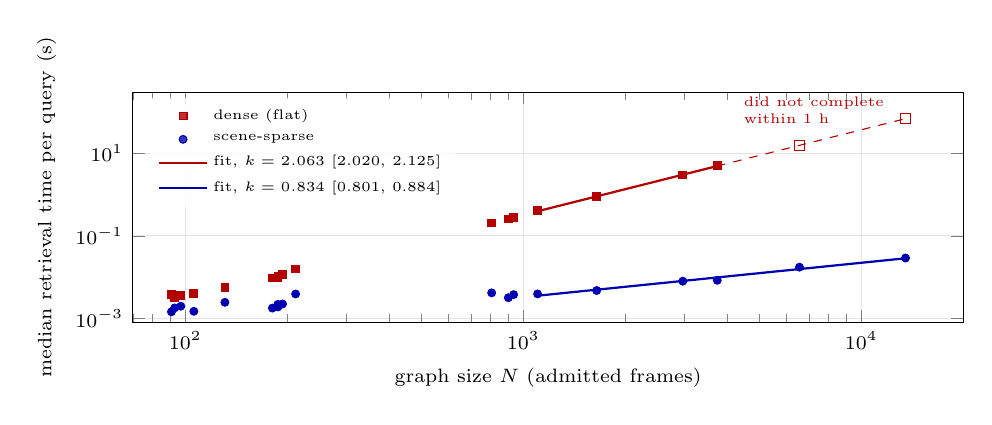
\begin{tikzpicture}
\begin{loglogaxis}[width=\columnwidth, height=4.5cm, font=\scriptsize,
  xlabel={graph size $N$ (admitted frames)}, ylabel={median retrieval time per query (s)},
  xmin=70, xmax=20000, ymin=8e-4, ymax=300,
  legend style={at={(0.02,0.98)}, anchor=north west, font=\tiny, draw=none, fill=white, fill opacity=0.8, text opacity=1},
  legend cell align=left, grid=major, grid style={gray!20}]
\addplot[only marks, mark=square*, mark size=1.4pt, red!70!black] coordinates {(91,0.0037804) (93,0.00323335) (97,0.0035986) (106,0.00405785) (131,0.0056776) (181,0.00950345) (188,0.00984055) (188,0.0104428) (194,0.0115663) (212,0.0156942) (806,0.20519) (903,0.256543) (936,0.27539) (1102,0.403426) (1648,0.881943) (2963,2.97617) (3747,5.05424)};
\addlegendentry{dense (flat)}
\addplot[only marks, mark=*, mark size=1.4pt, blue!70!black] coordinates {(91,0.00143485) (93,0.00178125) (97,0.00196115) (106,0.0014759) (131,0.0024339) (181,0.00176705) (188,0.00188595) (188,0.0021824) (194,0.00222335) (212,0.00388375) (806,0.00413525) (903,0.0031522) (936,0.00374655) (1102,0.0038955) (1648,0.0047096) (2963,0.007937) (3747,0.008328) (6559,0.0173718) (13506,0.0289635)};
\addlegendentry{scene-sparse}
\addplot[domain=1102:3747, samples=2, red!70!black, thick] {exp(-15.37917+2.062818*ln(x))};
\addlegendentry{fit, $k=2.063$ [2.020, 2.125]}
\addplot[domain=1102:13506, samples=2, blue!70!black, thick] {exp(-11.48851+0.833893*ln(x))};
\addlegendentry{fit, $k=0.834$ [0.801, 0.884]}
\addplot[domain=3747:13506, samples=2, red!70!black, dashed] {exp(-15.37917+2.062818*ln(x))};
\addplot[only marks, mark=square, mark size=1.8pt, red!70!black] coordinates {(6559,15.6) (13506,69.4)};
\node[font=\tiny, red!70!black, align=left, anchor=west] at (axis cs:4200,110) {did not complete\\within 1 h};
\end{loglogaxis}
\end{tikzpicture}
\Description{Log-log scatter of median retrieval time per query against graph size for the dense and scene-sparse arms, with fitted lines over graph sizes of 1102 and above. Dense points rise steeply to about 5 seconds at 3747 frames; its fitted line is extrapolated with a dashed segment, ending in two hollow markers at 6559 and 13506 frames where the dense measurement did not complete. Scene-sparse points stay between about 1 and 30 milliseconds.}
\caption{Query latency against graph size (19 UCF-Crime clips, real text queries), with the headline fits over $N\geq 1102$. Hollow markers are extrapolations where the dense measurement did not complete in an hour (\S5.2).}
\label{fig:scaling}
\end{figure}

Over the measured range (Figure~\ref{fig:scaling}), dense query cost grows with the square of graph size and
scene-sparse cost grows sublinearly. The headline fits (N \ensuremath{\geq} 1102) give k = 2.063 {[}2.020, 2.125{]} for dense
(4 clips, $R^2$ 0.999) and 0.834 {[}0.801, 0.884{]} for scene-sparse (6 clips, $R^2$ 0.983); over the full
range they give 1.980 {[}1.951, 2.006{]} (17 clips) and 0.497 {[}0.461, 0.530{]} (19 clips, $R^2$ 0.898).
The headline intervals are disjoint and the
scene-sparse upper bound lies below 1.0, the pre-registered bar for that separation.

We take as headline the less favourable sparse fit: the full-range 0.497 separates further,
but its poorer fit ($R^2$ 0.898 against 0.983) suggests a small-N noise floor, which we have not
verified directly. The dense arm is the complete graph the sparse one is pruned from; approximate
nearest-neighbour indexes are also sublinear, and we make no latency claim against them.

\textbf{Four caveats travel with the fit.}

\emph{Thin support at large N.} Against a target of five census clips per bin, N\ensuremath{\approx}1102 has 7, N\ensuremath{\approx}2963 has
2, N\ensuremath{\approx}6559 has 2 and N\ensuremath{\approx}13506 has 1; the survivor-N distribution is weighted toward small
graphs (census median N=333, with 24 of 31 census clips below N=1000). The headline fits rest on 4 dense
and 6 sparse points.

\emph{A guard violation, mechanism identified.} Two small-N clips (Assault036, N=97; Abuse037,
N=188) took the exact shortcut of §3.4 on 20\% and 10\% of queries, violating a pre-registered
guard that every timed query traverse PPR; its triggers grow likelier as scene count falls,
consistent with these being the two smallest clips. The shortcut degrades no result but is
faster, biasing the sparse arm favourably; both clips lie outside the headline range, and
excluding them raises the full-range exponent from 0.497 to 0.503, against us.

\emph{Salience-weight provenance.} The corpus was built throughout at salience weights
(\texttt{luma\_diff\_weight}, \texttt{motion\_weight}, \texttt{luma\_entropy\_weight}) = (0.5, 0.3, 0.2), verified
per-clip from cached configuration snapshots. Despite its name, \texttt{luma\_diff\_weight} weights a
codec \textbf{packet-size residual} (\texttt{frame\_features{[}"packet\_size"{]}}), not a luma-difference
quantity; a genuine \texttt{luma\_diff\_energy} field exists on frame records and is diagnostic only,
never consumed by the scorer. These are the shipped defaults, and they shape each survivor's
action score, not which frames survive (§3.1), so survivor counts do not depend on them.

\emph{Degree is flat against N, for this fit's edge mode only.} The exponent depends on per-scene
subgraphs not growing with N. Checked against all cached indices, degree does not drift
upward from N=24 to N=13,506 (r(N, deg\_mean) = \ensuremath{-}0.155), because scene count grows with N
(r=0.975) while scene size does not (r=0.135). This holds for the complete-block modes this
corpus is built under. It is \textbf{not} established at scale for the tiered mode our MLVU
results use: no cached index in this corpus was built under it, and the single tiered cache
measured since (one clip, N=613) confirms bounded degree there without establishing
degree-versus-N behaviour (§3).

\subsection{Behaviour at the largest sizes}

Each arm's measurement is one protocol under a uniform watchdog of 3600 s wall time and 29 GB
memory: graph build, then 253 timed queries. At N=6,559 (Arrest047) and N=13,506 (Arson019)
the dense arm exceeded the wall cap, with resident memory at 18.1 GB and 26.9 GB and still
rising when stopped; the scene-sparse arm completed both, at medians of 0.017 s and 0.029 s
per query.

The censoring is easy to overstate. The cap bounds the whole protocol, not one query, so these
runs do not show that a single dense query fails to return: extrapolating the §5.1 fit gives
roughly 16 s and 70 s per query, an extrapolation rather than a measurement. They do show cost
at the level of the graph. The dense graph at N=6,559 has 21.5 million edges, which at the
memory per edge measured at N=4,892 (about 690 bytes) accounts for the 18.1 GB observed, so it
was built and was being queried; at N=13,506 it has 91 million edges and would need roughly
64 GB, beyond this machine, consistent with a build still growing at the cap. We fit nothing to
these two clips and do not substitute the cap as a latency, since it bounds the protocol rather
than any query. (The scene-sparse arm's own peak here was 25.1 GB, because this run predates
block-diagonal construction and built its graph dense-then-prune --- the cost §4 removes.)

\subsection{End-to-end accounting: where the speedup goes}

Our own headline retrieval ratio buys nothing at the sizes we tested. We report it because
the literature reports retrieval-side speedups routinely and end-to-end accountings rarely.

Retrieval-\textbf{mechanics} measurements at N=4,892 show a 1,104\ensuremath{\times} ratio between arms (7.9448 s
dense against 0.0072 s scene-sparse) under synthetic sampled query embeddings. That
ratio does not reach the user, and it is a retrieval-mechanics figure wherever it appears.

We measured the full query path --- query text to final answer --- at the same N with
\texttt{granite4:micro} (\textasciitilde3.4B, Q4\_K\_M) on CPU, \texttt{l2\_retrieve\_top\_k=30}, five real CLIP-text queries
per arm plus a discarded warm-up, and the caption cache reset before each arm. The primary
run is instrumented on a clean checkout (pinned commit, zero tracked-dirty files). Stage medians,
dense against sparse: retrieval 8.535 against 0.030 s, captioning 37.27 against 62.13 s,
verification 6.41 against 4.42 s, answerer 2.83 s in both; totals 55.64 against 69.40 s.


Stage medians are taken independently, so they need not sum to the totals. \textbf{End-to-end
ratio: 0.802\ensuremath{\times} --- the sparse arm is slower at the median.} Per-query caption cost spans
2.6--69.3 s depending on cache misses, so at five queries per arm these medians are
directionally indicative rather than precise. An earlier measurement under a different
captioner gives 0.778\ensuremath{\times}; because captioning is 85--93\% of the dominant stage, the two runs
corroborate \textbf{direction only, not magnitude}.

Captioning is 85\% of the dominant stage in the dense arm and 93\% in the sparse arm. L1
retrieval costs exactly zero on every query in both arms --- it populates an in-memory
dictionary over already-retrieved frames --- so the stage is in practice a two-way split
between captioning and verification. Within it, frame access is not the cost: on one
cold-cache query at the same N (30 misses, 272 frames decoded, 27 distinct GOPs), the decode
loop cost 0.815 s against 114.6 s of captioning, under 1\% of the stage.

The retrieval ratio in this run is approximately 291\ensuremath{\times}, against the 1,104\ensuremath{\times} above. The two are
measured under different query types --- real CLIP text encoding here, synthetic embeddings
there --- and must not be conflated.

\textbf{The LLM is not the bottleneck:} the answerer costs 2.83 s in both arms. Captioning is
O(top\_k), not O(N), so sparsifying removes the retrieval term and leaves the largest untouched.

\textbf{Crossover.} The retrieval-only crossover --- the size past which scene-sparse retrieval
mechanics cost less than dense --- sits at N\ensuremath{\approx}24 from the §5.1 fits. We do not project an
end-to-end crossover. Doing so requires assuming the constant stage cost is equal across
arms, which this run's own data contradict (§5.4), and a projection built on that assumption
returns \textasciitilde1.15\ensuremath{\times} at N=4,892 where we measure 0.802\ensuremath{\times}. The large-N measurements of §5.2 are the
stronger statement, and we rest on them.

\subsection{Caption-cache locality (negative result)}

The sparse arm's captioning costs more than the dense arm's at identical top\_k. Over 20 real
text queries per arm at N=4,892, with top\_k verified byte-identical across arms (30 frames
on all 40 queries) and an identical query set, the paired clip-level bootstrap difference is
\textbf{+9.30 s per query, 95\% CI {[}3.52, 16.22{]}} (seed 42, B=10,000), excluding zero.

Per query, the sparse arm misses the caption cache 7.75 times against 3.85 and decodes 73.15
frames against 38.3, while per-frame caption time (2.520 s against 2.535 s) and verify calls
(1.00 against 1.05) are equal: the entire difference is miss count. We tested and
\textbf{rejected} the hypothesis that the sparse arm retrieves more temporally dispersed frames:
sparse retrievals touch marginally fewer distinct scenes (23.8 against 26.8), have a smaller
mean pairwise frame-index distance (2,732 against 3,070), and dispersion correlates
essentially not at all with caption time (pooled r = \ensuremath{-}0.058, n=40).

The mechanism is cross-query cache locality. The dense arm re-retrieves an overlapping pool
of high-salience frames largely independent of the query --- its miss count reaches zero by
the sixth distinct question --- whereas the sparse arm returns query-specific frames, so
successive questions touch largely disjoint frame sets and the cache warms slowly.

The dense arm's caching advantage thus comes from retrieval that is \emph{less responsive to the
query}. The cost is still real, since the cache persists across a session: the sparse graph
retrieves far more cheaply \emph{and} benefits less from caption reuse. Captioning
central frames before queries arrive could reduce it, at the cost of running a generative model
ahead of query time; we have not implemented or measured that.

\section{Correctness Floor}

This section does not claim competitive accuracy. It establishes two things: that the pipeline,
with no generative model in its construction path and a \textasciitilde3.4B answerer on CPU, answers
just below the weakly-supervised band; and that the cheap construction of §4 costs no
detectable grounded accuracy. §6.1 measures both on the official NExT-GQA test set; §6.2 uses
the tiered graph (§3.5).

\subsection{Grounded QA on NExT-GQA}

\textbf{A registered run on the official test set.} We evaluated all 5,553 questions over 990
videos of the official test split, which no earlier experiment of ours had touched, under a
pre-registration committed before any test video was downloaded, which fixed three
predictions and how each outcome would be reported. Three arms share one
ingest, captioner (MiniCPM-V 4.6, 1B) and answerer (\texttt{granite4:micro}, temperature 0, CPU):
\textbf{S}, the complete-block scene-sparse graph of §4; \textbf{F}, the flat graph; and \textbf{U},
twelve uniformly spaced frames. S and F retrieve twelve frames, and scoring uses the
benchmark's official convention. The run spanned six sessions, and every stop came from a guard
before any answer was affected (§8).

\begin{table}[t]
\footnotesize
\setlength{\tabcolsep}{4pt}
\caption{NExT-GQA official test set (5,553 questions). Our three rows share one captioner and answerer; their Acc@QA is 40.2 (S), 40.2 (F) and 43.2 (U).}
\begin{tabular}{llrrr}
\toprule
method & params & Acc@GQA & mIoP & IoP@0.5 \\
\midrule
Temp{[}CLIP{]} NG+ & 130M & 16.0 & 25.7 & 25.5 \\
SeViLA* & 4B & 16.6 & 29.5 & 22.9 \\
LangRepo & 8\ensuremath{\times}7B & 17.1 & 31.3 & 28.7 \\
FrozenBiLM NG+ & 1B & 17.5 & 24.2 & 23.7 \\
VideoMind-2B & 2B & 25.2 & 36.4 & 32.6 \\
MUPA-2B & 2B & 28.7 & 39.1 & 38.7 \\
MUPA-7B & 7B & 30.3 & 41.4 & 39.4 \\
\midrule
\textbf{IRIS-S}, scene-sparse & \textasciitilde3.4B, CPU & \textbf{13.8} & 29.9 & 30.7 \\
IRIS-F, flat & \textasciitilde3.4B, CPU & 13.5 & 28.9 & 29.7 \\
U, uniform frames & \textasciitilde3.4B, CPU & 5.2 & 21.7 & 9.3 \\
\bottomrule
\end{tabular}
\end{table}

\begin{figure}[t]
\centering
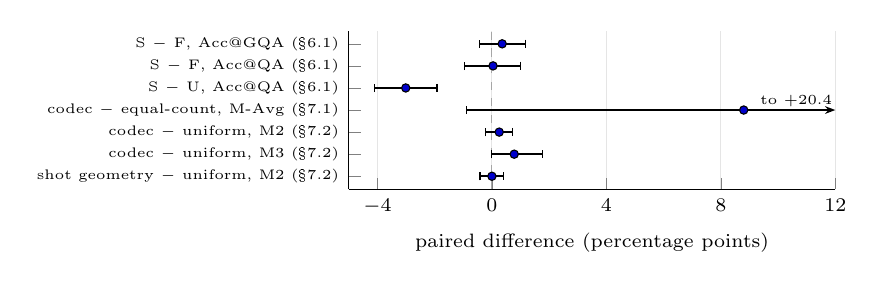
\begin{tikzpicture}
\begin{axis}[width=0.64\columnwidth, height=3.6cm, font=\scriptsize,
  xmin=-5, xmax=12, ymin=0.4, ymax=7.6, xtick={-4,0,4,8,12}, xlabel={paired difference (percentage points)},
  ytick={1,...,7}, yticklabel style={font=\tiny, align=right},
  yticklabels={{shot geometry $-$ uniform, M2 (\S7.2)},{codec $-$ uniform, M3 (\S7.2)},{codec $-$ uniform, M2 (\S7.2)},{codec $-$ equal-count, M-Avg (\S7.1)},{S $-$ U, Acc@QA (\S6.1)},{S $-$ F, Acc@QA (\S6.1)},{S $-$ F, Acc@GQA (\S6.1)}},
  xmajorgrids, grid style={gray!20}, axis y line*=left, axis x line*=bottom]
\draw[gray!70, dashed] (axis cs:0,0.4) -- (axis cs:0,7.6);
\draw[-{Stealth[length=1.3mm]}, line width=0.7pt] (axis cs:8.8,4) -- (axis cs:12,4);
\node[font=\tiny, anchor=south east, inner sep=1pt] at (axis cs:12,4) {to +20.4};
\addplot+[only marks, mark=*, mark size=1.5pt, black, error bars/.cd, x dir=both, x explicit, error bar style={line width=0.7pt}]
  coordinates {
  (0.36,7) += (0.81,0) -= (0.79,0)
  (0.04,6) += (0.97,0) -= (1.00,0)
  (-3.01,5) += (1.09,0) -= (1.08,0)
  (8.8,4) += (0,0) -= (9.7,0)
  (0.256,3) += (0.454,0) -= (0.492,0)
  (0.780,2) += (0.973,0) -= (0.785,0)
  (0.001,1) += (0.420,0) -= (0.417,0)
  };
\end{axis}
\end{tikzpicture}
\Description{Forest plot of seven paired differences with 95 percent confidence intervals, in percentage points, against a dashed zero line. Scene-sparse minus flat in grounded accuracy: plus 0.36, from minus 0.43 to plus 1.17. Scene-sparse minus flat in answer accuracy: plus 0.04, from minus 0.96 to plus 1.01. Scene-sparse minus uniform in answer accuracy: minus 3.01, from minus 4.09 to minus 1.92, the only interval excluding zero. Codec minus equal-count segmentation in M-Avg on long videos: plus 8.8, from minus 0.9 to plus 20.4. Codec admission minus uniform: M2 plus 0.256, from minus 0.236 to plus 0.710; M3 plus 0.780, from minus 0.005 to plus 1.753. Shot geometry minus uniform, M2: plus 0.001, from minus 0.416 to plus 0.421.}
\caption{All paired comparisons, with 95\% bootstrap intervals; only uniform's answer-accuracy lead excludes zero.}
\label{fig:forest}
\end{figure}

\textbf{The cheap construction costs no detectable accuracy (Figure~\ref{fig:forest}).} Paired over the same questions with a
video-clustered bootstrap (B=10,000), S\ensuremath{-}F is +0.0036 in Acc@GQA, 95\% CI {[}\ensuremath{-}0.0043, +0.0117{]},
and +0.0004 in Acc@QA, {[}\ensuremath{-}0.0096, +0.0101{]}. We report this as no detected change at
n=5,553, not as equivalence; the interval bounds any loss at 0.43 points of grounded accuracy.
This is the accuracy measurement §4's construction lacked.

\textbf{Two predictions failed.} We predicted Acc@GQA(S) between 0.14 and 0.19; it is 0.1385, just
below. We predicted retrieval would beat uniform sampling on answer accuracy; uniform is
better, Acc@QA S\ensuremath{-}U = \ensuremath{-}0.0301, 95\% CI {[}\ensuremath{-}0.0409, \ensuremath{-}0.0192{]}. Frames spread across the whole
video give the answerer broader context but rarely the evidence moment: U's IoP@0.5 is 0.093
against 0.307, so its grounded accuracy is 0.052 against 0.139. What retrieval contributes here
is grounding, not answers. Temporal questions fare worse than causal ones (Acc@GQA 0.096
against 0.169 for S).

\textbf{Grounding is the larger loss.} Acc@GQA(S) is P(grounded) = 0.307 times
P(correct \textbar{} grounded) = 0.450, and ungrounded questions are answered at 0.381 --- a 7-point
gap, against 15 on our validation carve. Perfect grounding would raise Acc@GQA to 0.450 (+0.31);
a perfect answerer over current grounding would give 0.307 (+0.17). F, which has no scene
shortlist, grounds no better (0.297), so the shortlist is not what limits grounding here.

\textbf{Both factors read one retrieval event.} \texttt{packet\_size} enters each arm's PageRank call
twice --- in the personalisation vector at weight (1\ensuremath{-}\ensuremath{\lambda})=0.5 and in the edge weights ---
and grounding and answering read the same retrieved frames. Grounding therefore shows that the
right evidence reached the answerer, not that the query found it for a semantic reason, and a
codec characteristic that favours retrieval while tracking question difficulty is not ruled out.

\textbf{Placement, and the earlier validation result.} Our rows use the published split and
scorer: S sits about 2 points below the weakest weakly-supervised row and 11--16 below the
agentic frontier, and we claim to beat nothing in the table. Before this run, a 120-question
held-out carve of the validation split (flat graph, union-convention scoring) gave Acc@GQA
0.1667, 95\% CI {[}0.088, 0.243{]}, consistent with the test result; there, retrieval led uniform
sampling in answer accuracy by +0.120 {[}0.000, 0.248{]}, a direction the test set reverses. That
carve is burned. One measurement touched it after it closed: an earlier run of §4.1's
equivalence check scored grounding on all 86 pool videos; nothing was tuned or selected from
it, and §4.1 reports a tuning-only re-run.

\subsection{Multi-task long-video QA on MLVU}

We also evaluate MLVU's~\cite{zhou2024mlvu} multiple-choice tasks, restricted to the six third-person ones: the
egocentric task is excluded because our compressed-domain signals assume a largely static
camera, and the generation tasks fall outside our multiple-choice harness. 150 questions, 25
per task, videos capped at 600 s, codec segmentation, scene-sparse graph.

\textbf{M-Avg 0.340}, zero ingest failures across 145 unique videos, overall option-parse failure
3.3\%.

\begin{table}[t]
\footnotesize
\setlength{\tabcolsep}{4pt}
\caption{MLVU per-task accuracy (150 questions, 25 per task).}
\begin{tabular}{lrrr}
\toprule
task & accuracy & chance & parse-fail \\
\midrule
Topic Reasoning & 0.720 & 0.250 & 4.0\% \\
Plot QA & 0.400 & 0.250 & 0.0\% \\
Anomaly Recognition & 0.320 & 0.250 & 0.0\% \\
Needle QA & 0.280 & 0.250 & 12.0\% \\
Action Order & 0.160 & 0.250 & 4.0\% \\
Action Count & 0.160 & 0.250 & 0.0\% \\
\bottomrule
\end{tabular}
\end{table}

\textbf{Two tasks fall below chance, and the cause is the answerer rather than retrieval.} Action
Order and Action Count sit at 0.160 against a 0.250 floor, with parse failure at 4\% and 0\%,
so the model is confidently wrong rather than unparsed. Both require what top-k retrieval
does not supply: chronological ordering needs reasoning over relative time, and exhaustive
counting needs complete coverage rather than the most relevant evidence. This is the same
failure mode as NExT-GQA's directional-temporal questions --- a limitation of the answerer at
this scale rather than of the graph (§8). Needle QA, with the highest parse-failure
rate (12\%), sits near chance, and we claim no margin there.

\subsection{What this section supports}

The system answers just below the band occupied by weakly-supervised methods with comparable
or larger models, on CPU with no training and no generative model in construction, and the
0.212 s construction of §4 costs it no detectable grounded accuracy.
Where it fails --- directional temporal reasoning, exhaustive counting --- the failure is in the
answerer rather than the representation.

\section{What Does Not Matter}

The results in this section are negative. We report them because each was tested against a
stated kill criterion, each criterion triggered, and together they delimit our own
contribution: they are why §4 claims \emph{cheap} construction rather than \emph{better} construction.
Both criteria were fixed before their runs, in dated records outside version control: §7.1's
in the task that commissioned the run, §7.2's in planning documents written before any run.
§7.2's scenario rule was tightened after a pilot, which we report where it matters.

\subsection{Segmentation placement, once the budget is fixed}

Our scene boundaries derive from compressed-domain residual peaks (§3.2). Does that
content-adaptive placement produce a better graph than a content-blind rule? We compared four
boundary strategies with retrieval, answerer, question set and seed held constant: \textbf{codec}
(residual peaks), \textbf{equal-count} and \textbf{equal-time} (both at the segment count codec produced
for that video, placed for equal survivor counts and equal intervals respectively), and
\textbf{fixed-60s}, the interval used by comparable pipelines. The matched-count arms isolate
\emph{where} boundaries fall from \emph{how many} there are.

On short videos (\ensuremath{\leq}600 s; six MLVU tasks, 150 questions, 145 videos) codec did not lead: M-Avg
0.340 codec, 0.393 equal-count, 0.320 equal-time, 0.353 fixed-60s --- the simplest matched-count
control 5.3 points ahead. Short videos yield few segments, so placement has little room to
matter; a long-video run (600--1800 s, AR and PQA, 45 videos) tests the regime where it should,
and the premise holds: codec produced a median of 581 scenes per video (range 174--1319)
against single digits on short videos.

Codec scores M-Avg 0.431 against equal-count's 0.343 (anomaly recognition 0.412 against 0.235,
n=17; plot QA 0.451 for both, n=91). The difference is \textbf{+0.088 M-Avg, 95\% CI {[}\ensuremath{-}0.009, +0.204{]}}
(video-clustered bootstrap, seed 42, B=10,000). The interval includes zero, the criterion
required it to exclude zero, and a tie was registered as failure. The difference did move in
the predicted direction (\ensuremath{-}0.053 on short videos to +0.088 on long), but all of it is carried
by anomaly recognition (+0.176, CI {[}0.000, 0.353{]}, n=17) while plot QA is exactly flat
(+0.000, CI {[}\ensuremath{-}0.101, +0.102{]}). \textbf{We therefore do not claim that codec-derived boundaries
produce a better graph.} A domain-concentrated benefit remains possible, untested at a sample
size that could resolve it.

The finding a practitioner should take: once the segment budget is fixed, boundary placement
is within noise across four strategies spanning content-adaptive to content-blind. That
licenses using the cheapest available segmentation, and it is a stronger argument for the
pipeline than a codec win would have been, because it does not depend on our signal being
special.

\subsection{Frame admission versus uniform sampling}

Do codec signals help \emph{select} which frames enter the graph? Three tests on the 19 annotated
UCF-Crime anomaly videos say they do not.

\textbf{Coverage metrics are uninformative without a matched control.} Uniform admission saturates
gold-window coverage (M1 = 1.0000) at every budget swept, down to 5\% retention, so any
selector appears to cover 99\%+ of gold windows: the metric measures annotated-window length,
not selection quality. We flag this because we previously reported such a figure ourselves.

\textbf{At matched budget, codec admission is indistinguishable from uniform.} At 10.5\% retention
the paired differences on the two informative metrics are +0.256 pp (95\% CI {[}\ensuremath{-}0.236, +0.710{]})
and +0.780 pp ({[}\ensuremath{-}0.005, +1.753{]}), both spanning zero; the admitted set sits at the
label-blind identity, mean(M2 \ensuremath{-} retention) = +0.0017 (sd 0.0099). Under the scenario rule as
first written, these positive point estimates would have counted as a win; a margin
requirement added after an n=8 pilot does not, and our claim rests on the intervals, which
span zero either way.

\textbf{Whether that tie reflects a wasted budget is unresolved.} A post-hoc diagnostic, not
pre-registered, found the codec top-k arm at k=503 sampling 42 distinct temporal locations
(8.4\% of budget) against uniform's 503, because the hold-forward-propagated action score is a
step function of about 9.5 frames per plateau and top-k takes whole plateaus. \textbf{This does
not dispose of the objection}: the diagnostic cannot separate an uninformative signal from a
budget spent on near-duplicates, and the plateau-dedup contrast that would is specified but not
run.

\textbf{Shot geometry adds nothing either.} Segmenting each video into shots directly from the
packet curve (zero decode) and sampling one frame per shot at its midpoint gives, against
uniform, +0.001 pp ({[}\ensuremath{-}0.416, +0.421{]}) and +0.141 pp ({[}\ensuremath{-}0.608, +0.972{]}) --- half-widths that
\emph{exclude} a 1 pp effect, making this the one properly powered contrast in the group and a
genuine null. The corresponding shot-plus-score contrast was underpowered (half-widths 1.69
and 2.79 pp) and we report it as such rather than as a tie.

\textbf{Power.} The annotated corpus is 19 videos, so each is 5.3 pp of any aggregate and the
resolution floor is roughly 1 pp; only more labelled anomaly footage changes that, and we did
not re-run in search of significance.

\subsection{What these negatives buy}

Neither \emph{where} we cut nor \emph{which frames we keep} is doing the work. What does is structural:
the graph is block-diagonal, so it is cheap to build and cheap to query, and that property is
independent of how the blocks are chosen --- narrower than the claim we set out to make, and
more portable. A pipeline adopting the construction needs the block structure, not our codec
signal, our segmentation, or our admission policy.

\section{Limitations}

Four constraints stated where they arose are indexed here: the retrieval speedup is
not an end-to-end speedup (0.802\ensuremath{\times}, §5.3); sparse retrieval pays a caption-cache penalty of
+9.30 s per query (§5.4); the scaling fit rests on 4 dense and 6 sparse points at large N
(§5.1); and accuracy sits just below the weakly-supervised band, 11--16 points below current
agentic methods (§6.1). The construction result carries no equivalent end-to-end caveat.

\textbf{The construction saving is measured on an evaluated configuration only for NExT-GQA.}
There, §6.1 detects no change in grounded accuracy. MLVU uses the tiered configuration, whose
neighbour selection scans all pairs regardless of how sparse its output is (§3.5, §4.3).
Bounding those scans to the scene partition would plausibly transfer the saving, but it yields
a different graph, so it needs accuracy validation rather than an identity proof.

\textbf{Directional temporal reasoning fails, and not in the graph.} Action Order and Action Count
fall below chance with near-zero parse failure, and NExT-GQA's before/after questions show the
same pattern (§6.1--§6.2). Both need relative temporal ordering or exhaustive coverage, which top-k
retrieval does not supply and which no change to graph construction addresses.

\textbf{Scene shortlisting bounds recall.} A scene excluded by the \(\lceil\sqrt{S}\rceil\)-width shortlist cannot
contribute evidence downstream (§3.4). Whether that width is recall-safe at large S is not
evaluated.

\textbf{Evaluation splits are constrained.} The NExT-GQA held-out \emph{validation} half is burned
(§6.1), which binds future answerer work more than the results reported here. MLVU is 150
questions across six tasks with videos capped at 600 s. The official NExT-GQA test split has now
been used once (§6.1); any further run on it is a second touch. Three further pre-registrations were
superseded before running or never run; we draw no evidence from them.

\textbf{Answerer reproducibility is scoped.} §6.1's test run re-answered 20 questions
byte-identically at the start of each of its six sessions, on its own llama-server build; the
earlier validation result is corroborated only by a 639/639 check on a different build and machine.
The MLVU results (§6.2, §7.1) ran through Ollama, whose client never sent the prompt-cache
disable flag and has no equivalent to single-slot serving, and every MLVU question was
answered exactly once, so \textbf{their reproducibility under re-query is undetermined}. §5.3--§5.4
also ran through Ollama, but report only timings and counts, which this does not affect.

\textbf{Encoding profiles are narrow.} A census of 200 UCF-Crime files finds 198 encoded with one
x264 setting --- one-pass ABR at 2000 kbps, keyframe interval 250, no B-frames --- and two
mislabelled MJPEG files outside our sets. On this corpus, then, ``always keep I-frames'' (§3.1)
amounts to periodic sampling every 250 frames, and every codec signal we read is a
second-generation measurement of an encoding history we did not control. The VIRAT efficiency
clip is \texttt{mpeg4}, and NExT-GQA's videos come from other, uncharacterised sources. The salience
channel, the codec-derived boundaries behind §4 and both negatives in §7 are conditioned on
these profiles; others are untested.

\textbf{Hardware and provenance.} The CPU-only claim rests on a \texttt{torch.cuda.is\_available()}
flag from a CPU-only wheel plus circumstantial path evidence; it shows that no CUDA device was
used, not that none was present. The zero-forward-pass claim (§3.1) is a property of the code
path and is unaffected. The \textasciitilde6.8\ensuremath{\times} memory ratio and the §5.1 exponents are not tied to a
clean commit, and the build-cost harness was committed after its run (§4.2).

\section{Conclusion}

We asked whether a long-video retrieval graph must be expensive to build. It need not be.
Block-diagonal construction produces exactly the graph that dense-then-prune produces while
visiting only the pairs it keeps: \textasciitilde234\ensuremath{\times} faster and \textasciitilde6.8\ensuremath{\times} smaller in memory on CPU,
with no generative model in the construction path. The same block structure separates query
latency into quadratic and sublinear regimes.

It does not make queries faster end to end, and accuracy sits just below the weakly-supervised
band, though the cheap graph costs no detectable grounded accuracy. Our two falsified hypotheses, on codec-derived boundaries and codec-based
admission (§7), show that neither where we cut nor which frames we keep does the work.
\textbf{The block structure alone does}, which is what makes the result portable. For retrieval
over long video, the intermediate graph does not have to be generated, and does not have to be
expensive. It has to be structured.

\begin{acks}
% DRAFT GenAI disclosure (ACM policy) -- all authors must approve the wording before submission.
The authors used a large language model assistant (Anthropic's Claude) to help audit experiment
provenance against code and artifacts, write analysis and run scripts, and draft and edit the
manuscript. The authors designed the experiments, ran them, verified every reported number
against its source artifact, and take full responsibility for the content.
\end{acks}

\bibliographystyle{ACM-Reference-Format}
\bibliography{refs_10pp}
\end{document}
